% Options for packages loaded elsewhere
% Options for packages loaded elsewhere
\PassOptionsToPackage{unicode}{hyperref}
\PassOptionsToPackage{hyphens}{url}
\PassOptionsToPackage{dvipsnames,svgnames,x11names}{xcolor}
%
\documentclass[
  norsk,
  a4paper,
]{article}
\usepackage{xcolor}
\usepackage{amsmath,amssymb}
\setcounter{secnumdepth}{3}
\usepackage{iftex}
\ifPDFTeX
  \usepackage[T1]{fontenc}
  \usepackage[utf8]{inputenc}
  \usepackage{textcomp} % provide euro and other symbols
\else % if luatex or xetex
  \usepackage{unicode-math} % this also loads fontspec
  \defaultfontfeatures{Scale=MatchLowercase}
  \defaultfontfeatures[\rmfamily]{Ligatures=TeX,Scale=1}
\fi
\usepackage{lmodern}
\ifPDFTeX\else
  % xetex/luatex font selection
\fi
% Use upquote if available, for straight quotes in verbatim environments
\IfFileExists{upquote.sty}{\usepackage{upquote}}{}
\IfFileExists{microtype.sty}{% use microtype if available
  \usepackage[]{microtype}
  \UseMicrotypeSet[protrusion]{basicmath} % disable protrusion for tt fonts
}{}
\makeatletter
\@ifundefined{KOMAClassName}{% if non-KOMA class
  \IfFileExists{parskip.sty}{%
    \usepackage{parskip}
  }{% else
    \setlength{\parindent}{0pt}
    \setlength{\parskip}{6pt plus 2pt minus 1pt}}
}{% if KOMA class
  \KOMAoptions{parskip=half}}
\makeatother
% Make \paragraph and \subparagraph free-standing
\makeatletter
\ifx\paragraph\undefined\else
  \let\oldparagraph\paragraph
  \renewcommand{\paragraph}{
    \@ifstar
      \xxxParagraphStar
      \xxxParagraphNoStar
  }
  \newcommand{\xxxParagraphStar}[1]{\oldparagraph*{#1}\mbox{}}
  \newcommand{\xxxParagraphNoStar}[1]{\oldparagraph{#1}\mbox{}}
\fi
\ifx\subparagraph\undefined\else
  \let\oldsubparagraph\subparagraph
  \renewcommand{\subparagraph}{
    \@ifstar
      \xxxSubParagraphStar
      \xxxSubParagraphNoStar
  }
  \newcommand{\xxxSubParagraphStar}[1]{\oldsubparagraph*{#1}\mbox{}}
  \newcommand{\xxxSubParagraphNoStar}[1]{\oldsubparagraph{#1}\mbox{}}
\fi
\makeatother


\usepackage{longtable,booktabs,array}
\newcounter{none} % for unnumbered tables
\usepackage{calc} % for calculating minipage widths
% Correct order of tables after \paragraph or \subparagraph
\usepackage{etoolbox}
\makeatletter
\patchcmd\longtable{\par}{\if@noskipsec\mbox{}\fi\par}{}{}
\makeatother
% Allow footnotes in longtable head/foot
\IfFileExists{footnotehyper.sty}{\usepackage{footnotehyper}}{\usepackage{footnote}}
\makesavenoteenv{longtable}
\usepackage{graphicx}
\makeatletter
\newsavebox\pandoc@box
\newcommand*\pandocbounded[1]{% scales image to fit in text height/width
  \sbox\pandoc@box{#1}%
  \Gscale@div\@tempa{\textheight}{\dimexpr\ht\pandoc@box+\dp\pandoc@box\relax}%
  \Gscale@div\@tempb{\linewidth}{\wd\pandoc@box}%
  \ifdim\@tempb\p@<\@tempa\p@\let\@tempa\@tempb\fi% select the smaller of both
  \ifdim\@tempa\p@<\p@\scalebox{\@tempa}{\usebox\pandoc@box}%
  \else\usebox{\pandoc@box}%
  \fi%
}
% Set default figure placement to htbp
\def\fps@figure{htbp}
\makeatother


% definitions for citeproc citations
\NewDocumentCommand\citeproctext{}{}
\NewDocumentCommand\citeproc{mm}{%
  \begingroup\def\citeproctext{#2}\cite{#1}\endgroup}
\makeatletter
 % allow citations to break across lines
 \let\@cite@ofmt\@firstofone
 % avoid brackets around text for \cite:
 \def\@biblabel#1{}
 \def\@cite#1#2{{#1\if@tempswa , #2\fi}}
\makeatother
\newlength{\cslhangindent}
\setlength{\cslhangindent}{1.5em}
\newlength{\csllabelwidth}
\setlength{\csllabelwidth}{3em}
\newenvironment{CSLReferences}[2] % #1 hanging-indent, #2 entry-spacing
 {\begin{list}{}{%
  \setlength{\itemindent}{0pt}
  \setlength{\leftmargin}{0pt}
  \setlength{\parsep}{0pt}
  % turn on hanging indent if param 1 is 1
  \ifodd #1
   \setlength{\leftmargin}{\cslhangindent}
   \setlength{\itemindent}{-1\cslhangindent}
  \fi
  % set entry spacing
  \setlength{\itemsep}{#2\baselineskip}}}
 {\end{list}}
\usepackage{calc}
\newcommand{\CSLBlock}[1]{\hfill\break\parbox[t]{\linewidth}{\strut\ignorespaces#1\strut}}
\newcommand{\CSLLeftMargin}[1]{\parbox[t]{\csllabelwidth}{\strut#1\strut}}
\newcommand{\CSLRightInline}[1]{\parbox[t]{\linewidth - \csllabelwidth}{\strut#1\strut}}
\newcommand{\CSLIndent}[1]{\hspace{\cslhangindent}#1}

\ifLuaTeX
\usepackage[bidi=basic,shorthands=off]{babel}
\else
\usepackage[bidi=default,shorthands=off]{babel}
\fi
\ifLuaTeX
  \usepackage{selnolig} % disable illegal ligatures
\fi


\setlength{\emergencystretch}{3em} % prevent overfull lines

\providecommand{\tightlist}{%
  \setlength{\itemsep}{0pt}\setlength{\parskip}{0pt}}



 


\usepackage{booktabs}
\usepackage{caption}
\usepackage{longtable}
\usepackage{colortbl}
\usepackage{array}
\usepackage{anyfontsize}
\usepackage{multirow}
\makeatletter
\@ifpackageloaded{caption}{}{\usepackage{caption}}
\AtBeginDocument{%
\ifdefined\contentsname
  \renewcommand*\contentsname{Innholdsfortegnelse}
\else
  \newcommand\contentsname{Innholdsfortegnelse}
\fi
\ifdefined\listfigurename
  \renewcommand*\listfigurename{Figurliste}
\else
  \newcommand\listfigurename{Figurliste}
\fi
\ifdefined\listtablename
  \renewcommand*\listtablename{Tabelliste}
\else
  \newcommand\listtablename{Tabelliste}
\fi
\ifdefined\figurename
  \renewcommand*\figurename{Figur}
\else
  \newcommand\figurename{Figur}
\fi
\ifdefined\tablename
  \renewcommand*\tablename{Tabell}
\else
  \newcommand\tablename{Tabell}
\fi
}
\@ifpackageloaded{float}{}{\usepackage{float}}
\floatstyle{ruled}
\@ifundefined{c@chapter}{\newfloat{codelisting}{h}{lop}}{\newfloat{codelisting}{h}{lop}[chapter]}
\floatname{codelisting}{Liste}
\newcommand*\listoflistings{\listof{codelisting}{Listeoversikt}}
\makeatother
\makeatletter
\makeatother
\makeatletter
\@ifpackageloaded{caption}{}{\usepackage{caption}}
\@ifpackageloaded{subcaption}{}{\usepackage{subcaption}}
\makeatother
\usepackage{bookmark}
\IfFileExists{xurl.sty}{\usepackage{xurl}}{} % add URL line breaks if available
\urlstyle{same}
% fallback for those not using the hyperref driver hyperxmp:
\makeatletter
\@ifundefined{xmpquote}{\newcommand{\xmpquote}[1]{#1}}{}
\makeatother
\hypersetup{
  pdftitle={Location{,} location{,} location? Hedoniske og romlige prismodeller for Lucas County{,} Ohio},
  pdflang={nb-NO},
  colorlinks=true,
  linkcolor={blue},
  filecolor={Maroon},
  citecolor={Blue},
  urlcolor={Blue},
  pdfcreator={LaTeX via pandoc}}


\title{Location, location, location? Hedoniske og romlige prismodeller
for Lucas County, Ohio}
\author{Harald Bjarne Vika \and Irjan A. Vikre \and Kristoffer Tufta}
\date{}
\begin{document}
\maketitle
\begin{abstract}
I dette term paperet analyserer vi 25 213 boligsalg i Lucas County,
Ohio, fra 1993--1998, koblet med sosioøkonomiske data fra American
Community Survey og miljødata fra EPAs EJScreen. Hedoniske OLS-modeller
viser at nabolaget betyr nesten like mye som boligen: forklaringskraften
øker fra 38,8 \% med bare boligkarakteristika til 74,7 \% når
beliggenhet, sosioøkonomiske forhold og miljøvariabler inkluderes.
Residualene er likevel sterkt romlig autokorrelerte (Moran's I mellom
0,32 og 0,37), og OLS gir derfor ikke et fullstendig bilde. Rao's
score-tester etter Anselin peker både mot SAR og SEM, mens LeSages
nestede likelihood ratio-tester entydig foretrekker Spatial Durbin Error
Model (SDEM), både med 3 og 10 nærmeste naboer. I SDEM er den direkte
elastisiteten for boligareal 0,55 og den totale 0,68, og en økning på 10
prosentpoeng i andelen svarte innbyggere er forbundet med om lag 7 \%
lavere boligpris. Valget av romlig modell påvirker de implisitte prisene
merkbart, og tolkningen av hedoniske estimater bør derfor ta hensyn til
romlige effekter.
\end{abstract}

\renewcommand*\contentsname{Innholdsfortegnelse}
{
\setcounter{tocdepth}{3}
\tableofcontents
}

\section{Oppgave 1}\label{oppgave-1}

\subsection{1.1 Laster inn og konverterer til
SF}\label{laster-inn-og-konverterer-til-sf}

\begin{verbatim}
[1] 25357    25
\end{verbatim}

\begin{verbatim}
[1] 2834
\end{verbatim}

\subsection{1.2 Lagger year-month}\label{lagger-year-month}

\begin{verbatim}
[1] "integer"
\end{verbatim}

\begin{verbatim}
[1] 960423 970421 931101 971223 950807 931101
\end{verbatim}

\begin{verbatim}
[1] "1993-01-04" "1998-10-05"
\end{verbatim}

\begin{verbatim}
[1] 70
\end{verbatim}

\begin{verbatim}

1993-01 1993-02 1993-03 1993-04 1993-05 1993-06 1993-07 1993-08 1993-09 1993-10 
    144     136     199     245     262     371     359     337     321     285 
1993-11 1993-12 1994-01 1994-02 1994-03 1994-04 1994-05 1994-06 1994-07 1994-08 
    316     285     194     172     268     317     384     417     351     373 
1994-09 1994-10 1994-11 1994-12 1995-01 1995-02 1995-03 1995-04 1995-05 1995-06 
    341     323     275     304     190     191     288     299     392     443 
1995-07 1995-08 1995-09 1995-10 1995-11 1995-12 1996-01 1996-02 1996-03 1996-04 
    412     469     394     407     347     298     232     249     320     474 
1996-05 1996-06 1996-07 1996-08 1996-09 1996-10 1996-11 1996-12 1997-01 1997-02 
    494     453     512     452     460     448     368     376     268     264 
1997-03 1997-04 1997-05 1997-06 1997-07 1997-08 1997-09 1997-10 1997-11 1997-12 
    351     457     511     487     493     493     450     461     348     449 
1998-01 1998-02 1998-03 1998-04 1998-05 1998-06 1998-07 1998-08 1998-09 1998-10 
    288     258     443     511     524     634     564     561     512      83 
\end{verbatim}

\subsection{1.3 CBD og Avstand}\label{cbd-og-avstand}

\begin{verbatim}
   Min. 1st Qu.  Median    Mean 3rd Qu.    Max. 
 0.1132  4.2355  6.8069  7.5892  9.5503 37.3821 
\end{verbatim}

\section{Oppgave 2}\label{oppgave-2}

\subsection{2.1 Leser inn variabler}\label{leser-inn-variabler}

\begin{verbatim}
[1] 398
\end{verbatim}

\subsection{2.2 Fjerner NA og fikser
projeksjon}\label{fjerner-na-og-fikser-projeksjon}

\begin{verbatim}
# A tibble: 1 x 14
  ID          LINGISOPCT LOWINCPCT LESSHSPCT OVER64PCT VULEOPCT PRE1960PCT PTRAF
  <chr>            <dbl>     <dbl>     <dbl>     <dbl>    <dbl>      <dbl> <dbl>
1 3909599000~          0         0         0         0        0          0    NA
# i 6 more variables: PWDIS <dbl>, PNPL <dbl>, PRMP <dbl>, PTSDF <dbl>,
#   OZONE <dbl>, PM25 <dbl>
\end{verbatim}

\begin{verbatim}
[1] 397
\end{verbatim}

\subsection{2.3 Fjerner vann}\label{fjerner-vann}

\begin{verbatim}
[1] 397
\end{verbatim}

\subsection{2.4 Kobler EJScreen opp mot
husdata}\label{kobler-ejscreen-opp-mot-husdata}

\begin{verbatim}
[1] 25357
\end{verbatim}

\begin{verbatim}
[1] 25352
\end{verbatim}

\begin{verbatim}
[1] 0
\end{verbatim}

\begin{verbatim}
[1] 5
\end{verbatim}

\section{Oppgave 3}\label{oppgave-3}

\subsection{Per Capita Inntekt}\label{per-capita-inntekt}

\begin{verbatim}
[1] 128
\end{verbatim}

\subsection{Etnisitet}\label{etnisitet}

\subsection{Pendletid}\label{pendletid}

\begin{verbatim}
# A tibble: 5 x 2
  GEOID        mwtt
  <chr>       <dbl>
1 39095000200  22.2
2 39095000300  19.3
3 39095000400  20.2
4 39095000600  21.2
5 39095000700  21.0
\end{verbatim}

\subsection{Medianinntekt pr. Hushold}\label{medianinntekt-pr.-hushold}

\subsection{Arbeidsstatus}\label{arbeidsstatus}

\subsection{Fattigdom}\label{fattigdom}

\subsection{Samlet datasett}\label{samlet-datasett}

\begin{verbatim}
        GEOID                                  NAME pc_inntekt andel_hvit
1 39095990000 Census Tract 9900, Lucas County, Ohio         NA        NaN
  andel_svart andel_asiatisk andel_andre andel_blandet mwtt median_hh_inntekt
1         NaN            NaN         NaN           NaN  NaN                NA
  andel_ledige fattig_under1 fattig_1til2 fattig_over2
1          NaN           NaN          NaN          NaN
\end{verbatim}

\begin{verbatim}
[1] 127
\end{verbatim}

\subsection{Projeksjon og vann}\label{projeksjon-og-vann}

\begin{verbatim}
[1] 127
\end{verbatim}

\begin{verbatim}
       GEOID            NAME       pc_inntekt      andel_hvit       
 Length   :127   Length   :127   Min.   : 4265   Min.   :0.0007321  
 N.unique :127   N.unique :127   1st Qu.:13750   1st Qu.:0.4649552  
 N.blank  :  0   N.blank  :  0   Median :21278   Median :0.8105288  
 Min.nchar: 11   Min.nchar: 34   Mean   :21699   Mean   :0.6847069  
 Max.nchar: 11   Max.nchar: 39   3rd Qu.:26795   3rd Qu.:0.9205472  
                                 Max.   :64170   Max.   :0.9983489  
                                                                    
  andel_svart      andel_asiatisk      andel_andre       andel_blandet     
 Min.   :0.00000   Min.   :0.000000   Min.   :0.000000   Min.   :0.000000  
 1st Qu.:0.03287   1st Qu.:0.000000   1st Qu.:0.004318   1st Qu.:0.007555  
 Median :0.10895   Median :0.004476   Median :0.011634   Median :0.024510  
 Mean   :0.25537   Mean   :0.012043   Mean   :0.019205   Mean   :0.028680  
 3rd Qu.:0.44960   3rd Qu.:0.018074   3rd Qu.:0.023475   3rd Qu.:0.040151  
 Max.   :0.97453   Max.   :0.076160   Max.   :0.137539   Max.   :0.137733  
                                                                           
      mwtt       median_hh_inntekt  andel_ledige     fattig_under1    
 Min.   :12.16   Min.   :  6717    Min.   :0.02469   Min.   :0.01493  
 1st Qu.:19.79   1st Qu.: 25897    1st Qu.:0.08523   1st Qu.:0.09171  
 Median :21.18   Median : 38438    Median :0.13307   Median :0.17480  
 Mean   :21.55   Mean   : 41615    Mean   :0.15789   Mean   :0.23501  
 3rd Qu.:23.15   3rd Qu.: 50607    3rd Qu.:0.19902   3rd Qu.:0.33886  
 Max.   :31.63   Max.   :113299    Max.   :0.67849   Max.   :0.86341  
                                                                      
  fattig_1til2      fattig_over2                                   tract_name 
 Min.   :0.02641   Min.   :0.08354   Census Tract 34, Lucas County, Ohio:  1  
 1st Qu.:0.13610   1st Qu.:0.36082   Census Tract 35, Lucas County, Ohio:  1  
 Median :0.20478   Median :0.59051   Census Tract 36, Lucas County, Ohio:  1  
 Mean   :0.20460   Mean   :0.56039   Census Tract 37, Lucas County, Ohio:  1  
 3rd Qu.:0.26334   3rd Qu.:0.73530   Census Tract 39, Lucas County, Ohio:  1  
 Max.   :0.50923   Max.   :0.92836   Census Tract 40, Lucas County, Ohio:  1  
                                     (Other)                            :121  
          geometry  
 MULTIPOLYGON : 14  
 POLYGON      :113  
 epsg:2834    :  0  
 +proj=lcc ...:  0  
                    
                    
                    
\end{verbatim}

\subsection{Kobler ACS til husdata}\label{kobler-acs-til-husdata}

\begin{verbatim}
[1] 25352
\end{verbatim}

\begin{verbatim}
[1] 25351
\end{verbatim}

\begin{verbatim}
[1] 0
\end{verbatim}

\begin{verbatim}
[1] 25351
\end{verbatim}

\subsection{Kontroll og lagring}\label{kontroll-og-lagring}

\begin{verbatim}
     price           yrbuilt         stories           TLA      
 Min.   :  2000   Min.   :1835   one     :12952   Min.   : 120  
 1st Qu.: 41900   1st Qu.:1924   bilevel :  508   1st Qu.:1070  
 Median : 65500   Median :1950   multilvl:  723   Median :1318  
 Mean   : 79013   Mean   :1945   one+half: 3123   Mean   :1462  
 3rd Qu.: 97000   3rd Qu.:1964   two     : 8041   3rd Qu.:1682  
 Max.   :875000   Max.   :1998   two+half:    2   Max.   :7616  
                                 three   :    2                 
       wall            beds           baths         halfbaths     
 stucdrvt:  204   Min.   :0.000   Min.   :0.000   Min.   :0.0000  
 ccbtile :  129   1st Qu.:3.000   1st Qu.:1.000   1st Qu.:0.0000  
 metlvnyl: 4235   Median :3.000   Median :1.000   Median :0.0000  
 brick   : 3632   Mean   :2.987   Mean   :1.242   Mean   :0.3412  
 stone   :   86   3rd Qu.:3.000   3rd Qu.:1.000   3rd Qu.:1.0000  
 wood    :11172   Max.   :9.000   Max.   :7.000   Max.   :3.0000  
 partbrk : 5893                                                   
    frontage          depth              garage        garagesqft    
 Min.   :  0.00   Min.   :   0.0   no garage: 3487   Min.   :   0.0  
 1st Qu.: 40.00   1st Qu.: 105.0   basement :   78   1st Qu.: 280.0  
 Median : 50.00   Median : 120.0   attached : 9016   Median : 396.0  
 Mean   : 64.27   Mean   : 119.1   detached :12552   Mean   : 369.5  
 3rd Qu.: 75.00   3rd Qu.: 140.0   carport  :  218   3rd Qu.: 484.0  
 Max.   :810.00   Max.   :1587.0                     Max.   :5755.0  
                                                                     
     rooms           lotsize           sdate            avalue      
 Min.   : 1.000   Min.   :   702   Min.   :930104   Min.   :  1714  
 1st Qu.: 5.000   1st Qu.:  4700   1st Qu.:941025   1st Qu.: 38514  
 Median : 6.000   Median :  6800   Median :960520   Median : 59714  
 Mean   : 6.115   Mean   : 13333   Mean   :957706   Mean   : 73636  
 3rd Qu.: 7.000   3rd Qu.: 11100   3rd Qu.:970818   3rd Qu.: 91114  
 Max.   :20.000   Max.   :429100   Max.   :981005   Max.   :788114  
                                                                    
     s1993            s1994            s1995            s1996       
 Min.   :0.0000   Min.   :0.0000   Min.   :0.0000   Min.   :0.0000  
 1st Qu.:0.0000   1st Qu.:0.0000   1st Qu.:0.0000   1st Qu.:0.0000  
 Median :0.0000   Median :0.0000   Median :0.0000   Median :0.0000  
 Mean   :0.1286   Mean   :0.1466   Mean   :0.1629   Mean   :0.1908  
 3rd Qu.:0.0000   3rd Qu.:0.0000   3rd Qu.:0.0000   3rd Qu.:0.0000  
 Max.   :1.0000   Max.   :1.0000   Max.   :1.0000   Max.   :1.0000  
                                                                    
     s1997            s1998         syear           age        
 Min.   :0.0000   Min.   :0.0000   1993:3259   Min.   :0.0100  
 1st Qu.:0.0000   1st Qu.:0.0000   1994:3716   1st Qu.:0.3500  
 Median :0.0000   Median :0.0000   1995:4130   Median :0.4900  
 Mean   :0.1985   Mean   :0.1727   1996:4837   Mean   :0.5366  
 3rd Qu.:0.0000   3rd Qu.:0.0000   1997:5032   3rd Qu.:0.7500  
 Max.   :1.0000   Max.   :1.0000   1998:4377   Max.   :1.6400  
                                                               
   sale_date            year_month       dist_CBD          house_id    
 Min.   :1993-01-04   1998-06:  633   Min.   : 0.1132   Min.   :    1  
 1st Qu.:1994-10-25   1998-07:  564   1st Qu.: 4.2351   1st Qu.: 6340  
 Median :1996-05-20   1998-08:  561   Median : 6.8051   Median :12677  
 Mean   :1996-03-19   1998-05:  524   Mean   : 7.5889   Mean   :12677  
 3rd Qu.:1997-08-18   1998-09:  512   3rd Qu.: 9.5518   3rd Qu.:19015  
 Max.   :1998-10-05   1996-07:  511   Max.   :37.3821   Max.   :25357  
                      (Other):22046                                    
         ID          LINGISOPCT         LOWINCPCT        LESSHSPCT      
 Length   :25351   Min.   :0.000000   Min.   :0.0000   Min.   :0.00000  
 N.unique :  386   1st Qu.:0.000000   1st Qu.:0.2118   1st Qu.:0.05350  
 N.blank  :    0   Median :0.000000   Median :0.3300   Median :0.08981  
 Min.nchar:   12   Mean   :0.009783   Mean   :0.3713   Mean   :0.11827  
 Max.nchar:   12   3rd Qu.:0.011057   3rd Qu.:0.5196   3rd Qu.:0.15870  
                   Max.   :0.150097   Max.   :0.9574   Max.   :0.57021  
                                                                        
   OVER64PCT          VULEOPCT         PRE1960PCT         PTRAF          
 Min.   :0.00000   Min.   :0.01092   Min.   :0.0000   Min.   :   0.8024  
 1st Qu.:0.08067   1st Qu.:0.15622   1st Qu.:0.2903   1st Qu.:  28.1792  
 Median :0.12742   Median :0.26347   Median :0.7022   Median :  67.3432  
 Mean   :0.13678   Mean   :0.31429   Mean   :0.6018   Mean   : 107.9907  
 3rd Qu.:0.17200   3rd Qu.:0.44744   3rd Qu.:0.8817   3rd Qu.: 125.5663  
 Max.   :0.53515   Max.   :0.93495   Max.   :1.0000   Max.   :1469.4353  
                                                                         
     PWDIS              PNPL               PRMP             PTSDF        
 Min.   :0.04950   Min.   :0.006919   Min.   :0.05877   Min.   :0.02420  
 1st Qu.:0.09322   1st Qu.:0.007943   1st Qu.:0.14413   1st Qu.:0.04550  
 Median :0.12717   Median :0.008327   Median :0.29217   Median :0.06252  
 Mean   :0.16815   Mean   :0.008275   Mean   :0.56705   Mean   :0.09585  
 3rd Qu.:0.18380   3rd Qu.:0.008624   3rd Qu.:1.01285   3rd Qu.:0.09295  
 Max.   :2.47212   Max.   :0.009063   Max.   :3.38001   Max.   :1.04588  
                                                                         
     OZONE            PM25             GEOID              NAME      
 Min.   :42.40   Min.   :10.36   Length   :25351   Length   :25351  
 1st Qu.:42.75   1st Qu.:10.75   N.unique :  124   N.unique :  124  
 Median :42.94   Median :10.83   N.blank  :    0   N.blank  :    0  
 Mean   :43.05   Mean   :10.81   Min.nchar:   11   Min.nchar:   34  
 3rd Qu.:43.28   3rd Qu.:10.89   Max.nchar:   11   Max.nchar:   39  
 Max.   :46.03   Max.   :10.96                                      
                                                                    
   pc_inntekt      andel_hvit         andel_svart      andel_asiatisk    
 Min.   : 4265   Min.   :0.0007321   Min.   :0.00000   Min.   :0.000000  
 1st Qu.:17386   1st Qu.:0.7003880   1st Qu.:0.02442   1st Qu.:0.000000  
 Median :22537   Median :0.8630722   Median :0.06829   Median :0.005563  
 Mean   :23617   Mean   :0.7734307   Mean   :0.16454   Mean   :0.013202  
 3rd Qu.:27895   3rd Qu.:0.9275962   3rd Qu.:0.22778   3rd Qu.:0.023140  
 Max.   :64170   Max.   :0.9983489   Max.   :0.97453   Max.   :0.076160  
                                                                         
  andel_andre       andel_blandet           mwtt       median_hh_inntekt
 Min.   :0.000000   Min.   :0.000000   Min.   :12.16   Min.   :  6717   
 1st Qu.:0.004902   1st Qu.:0.009401   1st Qu.:19.85   1st Qu.: 35603   
 Median :0.012815   Median :0.026038   Median :20.98   Median : 43929   
 Mean   :0.019150   Mean   :0.029672   Mean   :21.29   Mean   : 46395   
 3rd Qu.:0.024003   3rd Qu.:0.043881   3rd Qu.:22.49   3rd Qu.: 53822   
 Max.   :0.137539   Max.   :0.137733   Max.   :31.63   Max.   :113299   
                                                                        
  andel_ledige     fattig_under1      fattig_1til2      fattig_over2    
 Min.   :0.02469   Min.   :0.01493   Min.   :0.02641   Min.   :0.08354  
 1st Qu.:0.08164   1st Qu.:0.07192   1st Qu.:0.13615   1st Qu.:0.52190  
 Median :0.11029   Median :0.14300   Median :0.20478   Median :0.66289  
 Mean   :0.13322   Mean   :0.17895   Mean   :0.19674   Mean   :0.62431  
 3rd Qu.:0.17622   3rd Qu.:0.26308   3rd Qu.:0.25195   3rd Qu.:0.75363  
 Max.   :0.67849   Max.   :0.86341   Max.   :0.50923   Max.   :0.92836  
                                                                        
                                  tract_name             geometry    
 Census Tract 92.02, Lucas County, Ohio:  684   POINT        :25351  
 Census Tract 7, Lucas County, Ohio    :  644   epsg:2834    :    0  
 Census Tract 88, Lucas County, Ohio   :  480   +proj=lcc ...:    0  
 Census Tract 2, Lucas County, Ohio    :  409                        
 Census Tract 86, Lucas County, Ohio   :  406                        
 Census Tract 72.03, Lucas County, Ohio:  403                        
 (Other)                               :22325                        
\end{verbatim}

\begin{verbatim}
# A tibble: 0 x 2
# i 2 variables: variabel <chr>, antall_na <int>
\end{verbatim}

\begin{verbatim}
Deleting layer `Lucas County housing data' using driver `GPKG'
Writing layer `Lucas County housing data' to data source 
  `C:/Users/krist/Dev/Arbeidskrav-MSB205/Data/lucas_full.gpkg' using driver `GPKG'
Writing 25351 features with 57 fields and geometry type Point.
\end{verbatim}

\section{Oppgave 4}\label{oppgave-4}

\subsection{Utforskende dataanalyse}\label{sec-eda}

Før vi estimerer modellene, gjennomfører vi en utforskende romlig
dataanalyse (EDA) i GeoDa. Datasettet består av 25 351 boligsalg etter
koblingen med EJScreen- og ACS-dataene. Seks av de opprinnelige 25 357
observasjonene falt ut fordi de ikke lå innenfor noen av områdene etter
at vann var fjernet fra geometrien.

\subsubsection{Romlig fordeling av
prisene}\label{romlig-fordeling-av-prisene}

Salgsprisene varierer fra 2 000 til 875 000 dollar, med et gjennomsnitt
på om lag 79 000 dollar. Fordelingen er sterkt høyreskjev. De laveste
prisene er sannsynligvis ikke vanlige markedssalg.

Figur~\ref{fig-kvantil} viser prisene fordelt på fem kvantiler.
Mønsteret er tydelig: de billigste boligene ligger samlet i og rundt
Toledo sentrum, langs Maumee-elven og i de eldre bydelene nær sentrum.
De dyreste boligene ligger i forstedene, særlig nordvest mot Sylvania,
sørvest langs elven mot Maumee og Perrysburg og i de mer spredtbygde
områdene vest i fylket. Det finnes også en klynge av dyre boliger øst
for elven.

Prisene ser dermed ut til å øke med avstanden fra sentrum. Sammenhengen
er likevel ikke nødvendigvis lineær: prisene er lave nær sentrum, stiger
utover i forstedene og varierer mer i de ytterste, landlige områdene.
Dette er i tråd med den klassiske monosentriske bymodellen, men
mønsteret kan også gjenspeile at eldre og mindre boliger ligger nær
sentrum. Det er derfor viktig å kontrollere for boligkarakteristika når
vi estimerer effekten av avstand til CBD.

\begin{figure}[H]

\centering{

\pandocbounded{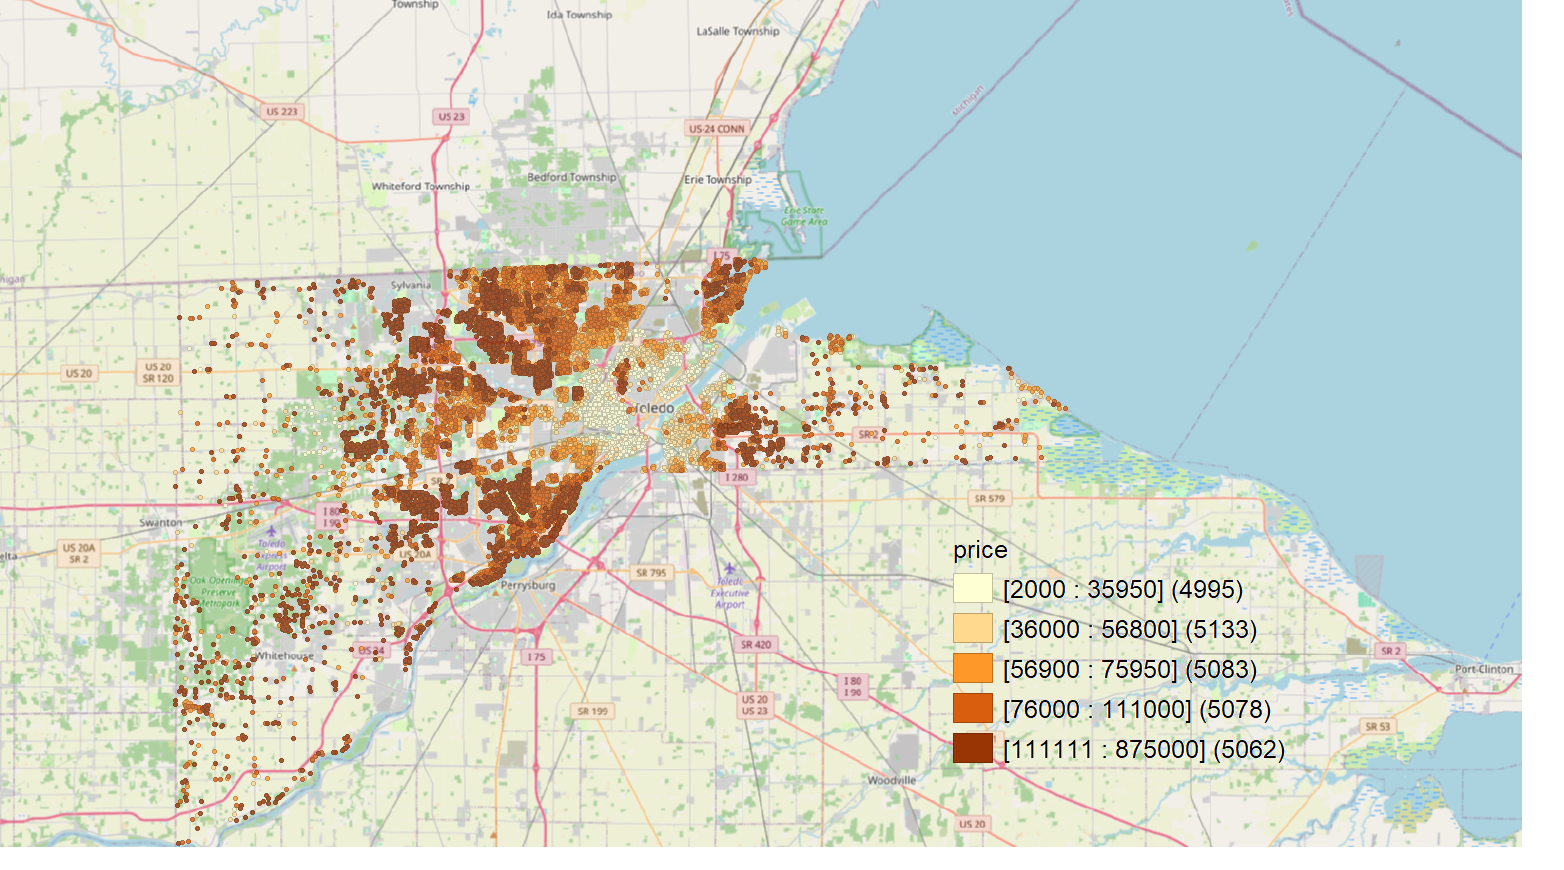
\includegraphics[keepaspectratio]{Data/lucas_county_price_qnt.png}}

}

\caption{\label{fig-kvantil}Salgspris for boliger i Lucas County,
1993--1998, fordelt på kvantiler.}

\end{figure}%

\subsubsection{Bivariat romlig autokorrelasjon mellom boligareal og
pris}\label{bivariat-romlig-autokorrelasjon-mellom-boligareal-og-pris}

For å undersøke hvordan boligens størrelse henger sammen med prisnivået
i nabolaget, bruker vi bivariat Moran's I med boligareal (\texttt{TLA})
som første variabel og salgspris (\texttt{price}) som andre. Den
bivariate statistikken måler sammenhengen mellom verdien av \texttt{TLA}
i et punkt og gjennomsnittet av \texttt{price} hos naboene, slik de er
definert i vektmatrisen. Vi bruker k-nærmeste-nabo-vekter med
henholdsvis k = 3 og k = 10.

Figur~\ref{fig-moran} viser Moran-plottene. Begge variablene er
standardisert. Den bivariate Moran's I er 0,646 med tre naboer
(Figur~\ref{fig-moran-k3}) og 0,619 med ti naboer
(Figur~\ref{fig-moran-k10}). Det er en sterk positiv sammenheng: store
boliger ligger typisk i nabolag med høye priser, og små boliger i
nabolag med lave priser. De fleste observasjonene ligger i kvadrantene
for høy-høy og lav-lav. En mindre andel ligger i de to andre
kvadrantene, altså små boliger i dyre nabolag og store boliger i billige
nabolag. Plottene viser også at begge variablene er høyreskjeve, med
enkelte svært store boliger og enkelte nabolag med svært høye priser.

At statistikken er noe lavere med ti naboer, er som forventet. Når
gjennomsnittet beregnes over flere naboer, jevnes ekstreme verdier ut,
og variasjonen i den laggede prisen blir mindre. Resultatet er likevel
robust for valget av k.

\begin{figure}[H]

\begin{minipage}[t]{0.50\linewidth}

\centering{

\pandocbounded{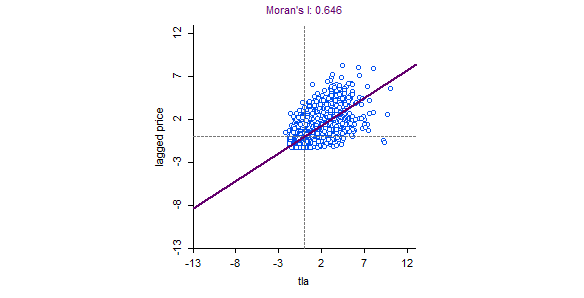
\includegraphics[keepaspectratio]{Data/lucas_county_BivMoransI_TLA_Price_k3.png}}

}

\subcaption{\label{fig-moran-k3}k = 3}

\end{minipage}%
%
\begin{minipage}[t]{0.50\linewidth}

\centering{

\pandocbounded{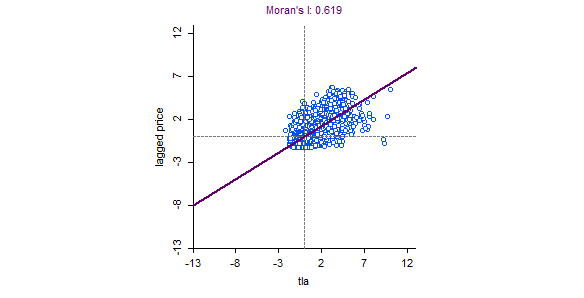
\includegraphics[keepaspectratio]{Data/lucas_county_BivMoransI_TLA_Price_k10.png}}

}

\subcaption{\label{fig-moran-k10}k = 10}

\end{minipage}%

\caption{\label{fig-moran}Bivariat Moran-plott for boligareal (TLA) og
laggede salgspriser. Begge variablene er standardisert.}

\end{figure}%

Figur~\ref{fig-bilisa} viser hvor de signifikante klyngene ligger.
Klynger av store og dyre boliger (høy-høy, 4 440 observasjoner) finner
vi i forstedene: nordvest mot Sylvania, sørvest langs elven mot Maumee,
i de spredtbygde områdene i vest rundt Whitehouse og i en klynge øst for
elven. Små og billige boliger (lav-lav, 6 928 observasjoner) er
konsentrert i Toledo sentrum og i bydelene nord og vest for sentrum.
Dette er den største gruppen.

De to blandede kategoriene er mindre, men interessante. Store boliger i
billige nabolag (høy-lav, 1 295 observasjoner) ligger spredt inne i
lav-lav-områdene nær sentrum og på østsiden av elven. Dette er trolig
eldre, store boliger i sentrumsnære bydeler der det generelle prisnivået
er lavt. Små boliger i dyre nabolag (lav-høy, 568 observasjoner) ligger
spredt i kantene av høy-høy-klyngene i forstedene. Om lag halvparten av
observasjonene (12 120) inngår ikke i noen signifikant klynge.

\begin{figure}[H]

\centering{

\pandocbounded{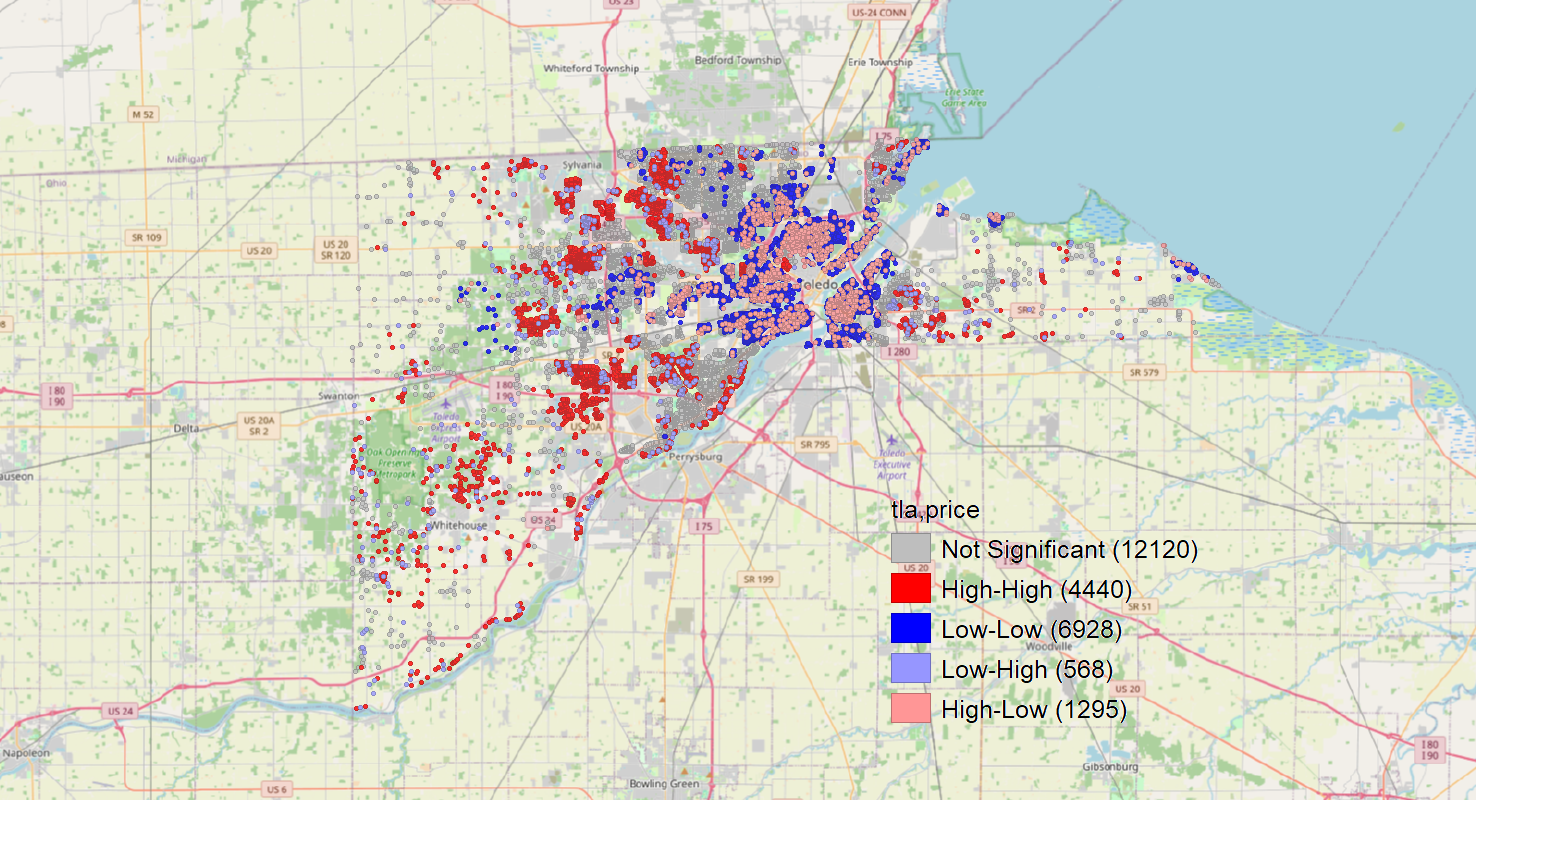
\includegraphics[keepaspectratio]{Data/lucas_county_price_LISA2.png}}

}

\caption{\label{fig-bilisa}Bivariat LISA-klyngekart for boligareal (TLA)
og salgspris, k = 10.}

\end{figure}%

\section{Oppgave 5}\label{oppgave-5}

\subsection{Lager datasett uten
geometridata}\label{lager-datasett-uten-geometridata}

\begin{verbatim}
     price           yrbuilt         stories           TLA      
 Min.   :  2000   Min.   :1835   one     :12952   Min.   : 120  
 1st Qu.: 41900   1st Qu.:1924   bilevel :  508   1st Qu.:1070  
 Median : 65500   Median :1950   multilvl:  723   Median :1318  
 Mean   : 79013   Mean   :1945   one+half: 3123   Mean   :1462  
 3rd Qu.: 97000   3rd Qu.:1964   two     : 8041   3rd Qu.:1682  
 Max.   :875000   Max.   :1998   two+half:    2   Max.   :7616  
                                 three   :    2                 
       wall            beds           baths         halfbaths     
 stucdrvt:  204   Min.   :0.000   Min.   :0.000   Min.   :0.0000  
 ccbtile :  129   1st Qu.:3.000   1st Qu.:1.000   1st Qu.:0.0000  
 metlvnyl: 4235   Median :3.000   Median :1.000   Median :0.0000  
 brick   : 3632   Mean   :2.987   Mean   :1.242   Mean   :0.3412  
 stone   :   86   3rd Qu.:3.000   3rd Qu.:1.000   3rd Qu.:1.0000  
 wood    :11172   Max.   :9.000   Max.   :7.000   Max.   :3.0000  
 partbrk : 5893                                                   
    frontage          depth              garage        garagesqft    
 Min.   :  0.00   Min.   :   0.0   no garage: 3487   Min.   :   0.0  
 1st Qu.: 40.00   1st Qu.: 105.0   basement :   78   1st Qu.: 280.0  
 Median : 50.00   Median : 120.0   attached : 9016   Median : 396.0  
 Mean   : 64.27   Mean   : 119.1   detached :12552   Mean   : 369.5  
 3rd Qu.: 75.00   3rd Qu.: 140.0   carport  :  218   3rd Qu.: 484.0  
 Max.   :810.00   Max.   :1587.0                     Max.   :5755.0  
                                                                     
     rooms           lotsize           sdate            avalue      
 Min.   : 1.000   Min.   :   702   Min.   :930104   Min.   :  1714  
 1st Qu.: 5.000   1st Qu.:  4700   1st Qu.:941025   1st Qu.: 38514  
 Median : 6.000   Median :  6800   Median :960520   Median : 59714  
 Mean   : 6.115   Mean   : 13333   Mean   :957706   Mean   : 73636  
 3rd Qu.: 7.000   3rd Qu.: 11100   3rd Qu.:970818   3rd Qu.: 91114  
 Max.   :20.000   Max.   :429100   Max.   :981005   Max.   :788114  
                                                                    
     s1993            s1994            s1995            s1996       
 Min.   :0.0000   Min.   :0.0000   Min.   :0.0000   Min.   :0.0000  
 1st Qu.:0.0000   1st Qu.:0.0000   1st Qu.:0.0000   1st Qu.:0.0000  
 Median :0.0000   Median :0.0000   Median :0.0000   Median :0.0000  
 Mean   :0.1286   Mean   :0.1466   Mean   :0.1629   Mean   :0.1908  
 3rd Qu.:0.0000   3rd Qu.:0.0000   3rd Qu.:0.0000   3rd Qu.:0.0000  
 Max.   :1.0000   Max.   :1.0000   Max.   :1.0000   Max.   :1.0000  
                                                                    
     s1997            s1998         syear           age        
 Min.   :0.0000   Min.   :0.0000   1993:3259   Min.   :0.0100  
 1st Qu.:0.0000   1st Qu.:0.0000   1994:3716   1st Qu.:0.3500  
 Median :0.0000   Median :0.0000   1995:4130   Median :0.4900  
 Mean   :0.1985   Mean   :0.1727   1996:4837   Mean   :0.5366  
 3rd Qu.:0.0000   3rd Qu.:0.0000   1997:5032   3rd Qu.:0.7500  
 Max.   :1.0000   Max.   :1.0000   1998:4377   Max.   :1.6400  
                                                               
   sale_date            year_month       dist_CBD          house_id    
 Min.   :1993-01-04   1998-06:  633   Min.   : 0.1132   Min.   :    1  
 1st Qu.:1994-10-25   1998-07:  564   1st Qu.: 4.2351   1st Qu.: 6340  
 Median :1996-05-20   1998-08:  561   Median : 6.8051   Median :12677  
 Mean   :1996-03-19   1998-05:  524   Mean   : 7.5889   Mean   :12677  
 3rd Qu.:1997-08-18   1998-09:  512   3rd Qu.: 9.5518   3rd Qu.:19015  
 Max.   :1998-10-05   1996-07:  511   Max.   :37.3821   Max.   :25357  
                      (Other):22046                                    
         ID          LINGISOPCT         LOWINCPCT        LESSHSPCT      
 Length   :25351   Min.   :0.000000   Min.   :0.0000   Min.   :0.00000  
 N.unique :  386   1st Qu.:0.000000   1st Qu.:0.2118   1st Qu.:0.05350  
 N.blank  :    0   Median :0.000000   Median :0.3300   Median :0.08981  
 Min.nchar:   12   Mean   :0.009783   Mean   :0.3713   Mean   :0.11827  
 Max.nchar:   12   3rd Qu.:0.011057   3rd Qu.:0.5196   3rd Qu.:0.15870  
                   Max.   :0.150097   Max.   :0.9574   Max.   :0.57021  
                                                                        
   OVER64PCT          VULEOPCT         PRE1960PCT         PTRAF          
 Min.   :0.00000   Min.   :0.01092   Min.   :0.0000   Min.   :   0.8024  
 1st Qu.:0.08067   1st Qu.:0.15622   1st Qu.:0.2903   1st Qu.:  28.1792  
 Median :0.12742   Median :0.26347   Median :0.7022   Median :  67.3432  
 Mean   :0.13678   Mean   :0.31429   Mean   :0.6018   Mean   : 107.9907  
 3rd Qu.:0.17200   3rd Qu.:0.44744   3rd Qu.:0.8817   3rd Qu.: 125.5663  
 Max.   :0.53515   Max.   :0.93495   Max.   :1.0000   Max.   :1469.4353  
                                                                         
     PWDIS              PNPL               PRMP             PTSDF        
 Min.   :0.04950   Min.   :0.006919   Min.   :0.05877   Min.   :0.02420  
 1st Qu.:0.09322   1st Qu.:0.007943   1st Qu.:0.14413   1st Qu.:0.04550  
 Median :0.12717   Median :0.008327   Median :0.29217   Median :0.06252  
 Mean   :0.16815   Mean   :0.008275   Mean   :0.56705   Mean   :0.09585  
 3rd Qu.:0.18380   3rd Qu.:0.008624   3rd Qu.:1.01285   3rd Qu.:0.09295  
 Max.   :2.47212   Max.   :0.009063   Max.   :3.38001   Max.   :1.04588  
                                                                         
     OZONE            PM25             GEOID              NAME      
 Min.   :42.40   Min.   :10.36   Length   :25351   Length   :25351  
 1st Qu.:42.75   1st Qu.:10.75   N.unique :  124   N.unique :  124  
 Median :42.94   Median :10.83   N.blank  :    0   N.blank  :    0  
 Mean   :43.05   Mean   :10.81   Min.nchar:   11   Min.nchar:   34  
 3rd Qu.:43.28   3rd Qu.:10.89   Max.nchar:   11   Max.nchar:   39  
 Max.   :46.03   Max.   :10.96                                      
                                                                    
   pc_inntekt      andel_hvit         andel_svart      andel_asiatisk    
 Min.   : 4265   Min.   :0.0007321   Min.   :0.00000   Min.   :0.000000  
 1st Qu.:17386   1st Qu.:0.7003880   1st Qu.:0.02442   1st Qu.:0.000000  
 Median :22537   Median :0.8630722   Median :0.06829   Median :0.005563  
 Mean   :23617   Mean   :0.7734307   Mean   :0.16454   Mean   :0.013202  
 3rd Qu.:27895   3rd Qu.:0.9275962   3rd Qu.:0.22778   3rd Qu.:0.023140  
 Max.   :64170   Max.   :0.9983489   Max.   :0.97453   Max.   :0.076160  
                                                                         
  andel_andre       andel_blandet           mwtt       median_hh_inntekt
 Min.   :0.000000   Min.   :0.000000   Min.   :12.16   Min.   :  6717   
 1st Qu.:0.004902   1st Qu.:0.009401   1st Qu.:19.85   1st Qu.: 35603   
 Median :0.012815   Median :0.026038   Median :20.98   Median : 43929   
 Mean   :0.019150   Mean   :0.029672   Mean   :21.29   Mean   : 46395   
 3rd Qu.:0.024003   3rd Qu.:0.043881   3rd Qu.:22.49   3rd Qu.: 53822   
 Max.   :0.137539   Max.   :0.137733   Max.   :31.63   Max.   :113299   
                                                                        
  andel_ledige     fattig_under1      fattig_1til2      fattig_over2    
 Min.   :0.02469   Min.   :0.01493   Min.   :0.02641   Min.   :0.08354  
 1st Qu.:0.08164   1st Qu.:0.07192   1st Qu.:0.13615   1st Qu.:0.52190  
 Median :0.11029   Median :0.14300   Median :0.20478   Median :0.66289  
 Mean   :0.13322   Mean   :0.17895   Mean   :0.19674   Mean   :0.62431  
 3rd Qu.:0.17622   3rd Qu.:0.26308   3rd Qu.:0.25195   3rd Qu.:0.75363  
 Max.   :0.67849   Max.   :0.86341   Max.   :0.50923   Max.   :0.92836  
                                                                        
                                  tract_name      log_price     
 Census Tract 92.02, Lucas County, Ohio:  684   Min.   : 7.601  
 Census Tract 7, Lucas County, Ohio    :  644   1st Qu.:10.643  
 Census Tract 88, Lucas County, Ohio   :  480   Median :11.090  
 Census Tract 2, Lucas County, Ohio    :  409   Mean   :11.020  
 Census Tract 86, Lucas County, Ohio   :  406   3rd Qu.:11.482  
 Census Tract 72.03, Lucas County, Ohio:  403   Max.   :13.682  
 (Other)                               :22325                   
\end{verbatim}

\subsection{Hedoniske modeller}\label{hedoniske-modeller}

For å undersøke hvilke faktorer som påvirker boligprisene i Lucas
County, estimeres tre hedoniske boligprismodeller med et gradvis utvidet
sett av forklaringsvariabler. Modellvalgene tar utgangspunkt i
Maslianskaia-Pautrel \& Baumont (2016), som undersøker hvordan
boligpriser påvirkes av boligens egenskaper, geografisk beliggenhet og
miljørelaterte forhold. Forfatterne bygger på hedonisk pristeori, hvor
boligprisen betraktes som et resultat av flere ulike egenskaper ved
boligen og dens omgivelser.

\subsubsection{Modell 1}\label{modell-1}

Den første modellen fungerer som en grunnmodell og inkluderer boligens
egne karakteristika, samt tidsdummyer for år og måned. Boligareal (TLA)
er en sentral forklaringsvariabel, ettersom større boliger normalt
forventes å ha høyere salgspris. Andre relevante boligkarakteristika bør
også inkluderes for å kontrollere for forskjeller i boligenes fysiske
egenskaper.

Dette er i tråd med Maslianskaia-Pautrel \& Baumont (2016), som
beskriver boligprisen som en funksjon av både boligegenskaper og forhold
knyttet til beliggenheten. Ved å starte med boligkarakteristika kan vi
undersøke hvor mye av prisvariasjonen som kan forklares av selve
boligen, før vi inkluderer forhold ved området den ligger i
(Maslianskaia-Pautrel \& Baumont, 2016, s. 923--924).

Tidsdummyene inkluderes for å kontrollere for mulige endringer i det
generelle boligprisnivået gjennom perioden 1993--1998. Dette gjør det
mulig å skille mellom prisforskjeller som skyldes boligens egenskaper og
prisforskjeller knyttet til tidspunktet for salget.

\subsubsection{Modell 2}\label{modell-2}

Den andre modellen utvider grunnmodellen med avstand til sentrum
(dist\_CBD) og demografiske og sosioøkonomiske variabler fra ACS5 og
EJScreen. Dette inkluderer blant annet inntektsnivå, arbeidsledighet,
befolkningssammensetning og gjennomsnittlig reisetid til arbeid.

Maslianskaia-Pautrel \& Baumont (2016) understreker at boligens
beliggenhet og tilgjengelighet til ulike områder og fasiliteter kan ha
betydning for boligverdien. På bakgrunn av dette inkluderes avstanden
til Toledos sentrum som et mål på geografisk tilgjengelighet. Avstand
til sentrum kan påvirke boligprisene gjennom blant annet
transportkostnader og nærhet til arbeidsplasser og tjenester.
Sammenhengen trenger imidlertid ikke å være negativ, ettersom boligene i
forstedene også kan være større eller ligge i mer attraktive
boligområder (Maslianskaia-Pautrel \& Baumont, 2016, s. 924).

De sosioøkonomiske variablene inkluderes for å kontrollere for
forskjeller mellom nabolagene. Inntektsnivå og arbeidsledighet kan
eksempelvis gjenspeile lokale økonomiske forhold, mens
befolkningssammensetningen kan fange opp forskjeller mellom boligområder
som ikke forklares av boligens fysiske egenskaper alene. Disse
variablene bør tolkes som indikatorer på nabolagsforhold, og ikke
nødvendigvis som direkte årsaker til boligprisforskjeller.

Formålet med modell 2 er dermed å undersøke om områdeforhold bidrar til
å forklare boligprisene utover det som allerede forklares av
boligkarakteristika og tidspunktet for salget.

\subsubsection{Modell 3}\label{modell-3}

Den tredje modellen utvider modell 2 ved å inkludere miljørelaterte
variabler fra EJScreen. Variablene omfatter blant annet
trafikkbelastning (PTRAF), nærhet til forurensede områder (PNPL),
luftforurensning (PM25) og andelen eldre boliger (PRE1960PCT).

Dette modellvalget er særlig relevant med utgangspunkt i
Maslianskaia-Pautrel \& Baumont (2016), som undersøker hvordan
miljømessige kvaliteter og ulemper påvirker boligpriser. Forfatterne
viser til at miljøforhold som trafikkstøy, forurensning og nærhet til
industriområder kan inngå i boligkjøpernes vurdering av en eiendom.

Miljøvariablene inkluderes derfor for å undersøke om slike forhold har
en selvstendig sammenheng med boligprisene når vi allerede har
kontrollert for boligkarakteristika, beliggenhet og sosioøkonomiske
forhold. Det kan eksempelvis forventes at høyere miljøbelastning er
forbundet med lavere boligpriser, men den faktiske sammenhengen må
undersøkes empirisk.

Maslianskaia-Pautrel \& Baumont (2016) fremhever også betydningen av
romlige effekter. Miljøforhold kan påvirke flere nærliggende boliger
samtidig, og boligprisene kan være påvirket av forhold i omkringliggende
områder. Dette innebærer at en vanlig OLS-modell ikke nødvendigvis
fanger opp alle geografiske sammenhenger (Maslianskaia-Pautrel \&
Baumont, 2016, s. 925--927).

\subsection{Vurdering av modellene}\label{vurdering-av-modellene}

Ved å estimere tre modeller med gradvis flere forklaringsvariabler kan
vi undersøke hvordan sammenhengen mellom boligpris og de ulike
egenskapene endres når flere forhold kontrolleres for. Modell 1 gir et
utgangspunkt basert på boligkarakteristika, modell 2 inkluderer
geografiske og sosioøkonomiske forhold, mens modell 3 også undersøker
betydningen av miljøbelastning.

Modellene sammenlignes ved hjelp av blant annet justert R², AIC og
koeffisientenes statistiske signifikans. En forbedring i
modelltilpasningen ved inkludering av flere variabler kan indikere at
disse bidrar til å forklare variasjonen i boligprisene. Samtidig må
modellvalget vurderes ut fra økonomisk teori og risikoen for
multikollinearitet.

Et viktig poeng fra Maslianskaia-Pautrel \& Baumont (2016) er at
boligpriser og miljøforhold kan være romlig avhengige. De tre
OLS-modellene gir derfor et grunnlag for videre undersøkelser av romlig
autokorrelasjon og eventuelle romlige regresjonsmodeller senere i
oppgaven.

\begin{verbatim}

    studentized Breusch-Pagan test

data:  modell1
BP = 226.7, df = 70, p-value < 2.2e-16
\end{verbatim}

\begin{verbatim}

    studentized Breusch-Pagan test

data:  modell2
BP = 2636.5, df = 78, p-value < 2.2e-16
\end{verbatim}

\begin{verbatim}

    studentized Breusch-Pagan test

data:  modell3
BP = 2725.9, df = 82, p-value < 2.2e-16
\end{verbatim}

\subsection{Regresjonsmodell}\label{regresjonsmodell}

\begin{table}
\fontsize{12.0pt}{14.0pt}\selectfont
\begin{tabular*}{\linewidth}{@{\extracolsep{\fill}}lccc}
\toprule
  & Modell 1 & Modell 2 & Modell 3 \\ 
\midrule\addlinespace[2.5pt]
(Intercept) & 1.605*** & 5.885*** & -6.550*** \\ 
 & (17.277) & (81.001) & (-6.279) \\ 
log(TLA) & 1.273*** & 0.801*** & 0.754*** \\ 
 & (123.097) & (91.161) & (85.022) \\ 
year\_month1993-02 & -0.105 & -0.072 & -0.059 \\ 
 & (-1.314) & (-1.373) & (-1.152) \\ 
year\_month1993-03 & 0.107 & 0.009 & 0.022 \\ 
 & (1.581) & (0.208) & (0.548) \\ 
year\_month1993-04 & 0.044 & -0.020 & -0.008 \\ 
 & (0.651) & (-0.499) & (-0.221) \\ 
year\_month1993-05 & 0.205*** & 0.101** & 0.101** \\ 
 & (3.329) & (2.695) & (2.765) \\ 
year\_month1993-06 & 0.145* & 0.017 & 0.035 \\ 
 & (2.389) & (0.482) & (1.001) \\ 
year\_month1993-07 & 0.170** & 0.027 & 0.042 \\ 
 & (2.768) & (0.756) & (1.211) \\ 
year\_month1993-08 & 0.129* & 0.049 & 0.052 \\ 
 & (2.065) & (1.316) & (1.471) \\ 
year\_month1993-09 & 0.152* & 0.053 & 0.066+ \\ 
 & (2.436) & (1.436) & (1.852) \\ 
year\_month1993-10 & 0.170** & 0.077* & 0.078* \\ 
 & (2.664) & (2.040) & (2.137) \\ 
year\_month1993-11 & 0.211*** & 0.080* & 0.086* \\ 
 & (3.465) & (2.174) & (2.422) \\ 
year\_month1993-12 & 0.197** & 0.069+ & 0.070+ \\ 
 & (3.121) & (1.831) & (1.939) \\ 
year\_month1994-01 & 0.158* & 0.078* & 0.084* \\ 
 & (2.371) & (2.014) & (2.233) \\ 
year\_month1994-02 & 0.076 & 0.015 & 0.018 \\ 
 & (1.041) & (0.341) & (0.439) \\ 
year\_month1994-03 & 0.141* & 0.045 & 0.046 \\ 
 & (2.199) & (1.168) & (1.247) \\ 
year\_month1994-04 & 0.200** & 0.090* & 0.100** \\ 
 & (3.241) & (2.436) & (2.803) \\ 
year\_month1994-05 & 0.223*** & 0.078* & 0.081* \\ 
 & (3.643) & (2.130) & (2.300) \\ 
year\_month1994-06 & 0.200** & 0.069+ & 0.073* \\ 
 & (3.273) & (1.905) & (2.093) \\ 
year\_month1994-07 & 0.215*** & 0.093** & 0.093** \\ 
 & (3.547) & (2.625) & (2.718) \\ 
year\_month1994-08 & 0.252*** & 0.150*** & 0.157*** \\ 
 & (4.148) & (4.125) & (4.481) \\ 
year\_month1994-09 & 0.148* & 0.057 & 0.072* \\ 
 & (2.378) & (1.548) & (2.006) \\ 
year\_month1994-10 & 0.172** & 0.085* & 0.090* \\ 
 & (2.711) & (2.290) & (2.476) \\ 
year\_month1994-11 & 0.145* & 0.093* & 0.108** \\ 
 & (2.207) & (2.342) & (2.831) \\ 
year\_month1994-12 & 0.069 & 0.006 & 0.021 \\ 
 & (1.037) & (0.148) & (0.565) \\ 
year\_month1995-01 & 0.103 & 0.082+ & 0.087* \\ 
 & (1.422) & (1.854) & (2.061) \\ 
year\_month1995-02 & 0.076 & 0.042 & 0.059 \\ 
 & (1.059) & (1.018) & (1.499) \\ 
year\_month1995-03 & 0.158* & 0.109** & 0.111** \\ 
 & (2.435) & (2.820) & (2.977) \\ 
year\_month1995-04 & 0.186** & 0.112** & 0.119*** \\ 
 & (2.888) & (2.948) & (3.301) \\ 
year\_month1995-05 & 0.217*** & 0.145*** & 0.152*** \\ 
 & (3.545) & (3.972) & (4.319) \\ 
year\_month1995-06 & 0.256*** & 0.146*** & 0.151*** \\ 
 & (4.288) & (4.098) & (4.391) \\ 
year\_month1995-07 & 0.240*** & 0.121*** & 0.133*** \\ 
 & (3.992) & (3.352) & (3.844) \\ 
year\_month1995-08 & 0.254*** & 0.141*** & 0.148*** \\ 
 & (4.249) & (4.013) & (4.360) \\ 
year\_month1995-09 & 0.261*** & 0.138*** & 0.159*** \\ 
 & (4.333) & (3.868) & (4.586) \\ 
year\_month1995-10 & 0.219*** & 0.107** & 0.117*** \\ 
 & (3.585) & (2.925) & (3.293) \\ 
year\_month1995-11 & 0.210*** & 0.119** & 0.133*** \\ 
 & (3.320) & (3.216) & (3.725) \\ 
year\_month1995-12 & 0.203** & 0.128*** & 0.142*** \\ 
 & (3.166) & (3.316) & (3.808) \\ 
year\_month1996-01 & 0.108 & 0.046 & 0.055 \\ 
 & (1.599) & (1.097) & (1.399) \\ 
year\_month1996-02 & 0.167* & 0.084* & 0.102** \\ 
 & (2.462) & (2.079) & (2.647) \\ 
year\_month1996-03 & 0.316*** & 0.171*** & 0.166*** \\ 
 & (5.103) & (4.421) & (4.397) \\ 
year\_month1996-04 & 0.292*** & 0.167*** & 0.177*** \\ 
 & (4.887) & (4.696) & (5.136) \\ 
year\_month1996-05 & 0.285*** & 0.146*** & 0.150*** \\ 
 & (4.776) & (4.075) & (4.327) \\ 
year\_month1996-06 & 0.291*** & 0.176*** & 0.182*** \\ 
 & (4.782) & (4.842) & (5.168) \\ 
year\_month1996-07 & 0.250*** & 0.155*** & 0.169*** \\ 
 & (4.133) & (4.271) & (4.790) \\ 
year\_month1996-08 & 0.248*** & 0.130*** & 0.139*** \\ 
 & (4.038) & (3.482) & (3.870) \\ 
year\_month1996-09 & 0.157* & 0.088* & 0.091* \\ 
 & (2.522) & (2.245) & (2.411) \\ 
year\_month1996-10 & 0.188** & 0.106** & 0.113** \\ 
 & (2.970) & (2.751) & (3.023) \\ 
year\_month1996-11 & 0.210** & 0.125** & 0.130*** \\ 
 & (3.262) & (3.070) & (3.323) \\ 
year\_month1996-12 & 0.171** & 0.063 & 0.073+ \\ 
 & (2.642) & (1.532) & (1.842) \\ 
year\_month1997-01 & 0.062 & 0.036 & 0.041 \\ 
 & (0.890) & (0.808) & (0.964) \\ 
year\_month1997-02 & 0.175* & 0.105* & 0.099* \\ 
 & (2.542) & (2.482) & (2.446) \\ 
year\_month1997-03 & 0.192** & 0.103* & 0.111** \\ 
 & (2.972) & (2.522) & (2.835) \\ 
year\_month1997-04 & 0.226*** & 0.143*** & 0.148*** \\ 
 & (3.635) & (3.716) & (3.987) \\ 
year\_month1997-05 & 0.266*** & 0.148*** & 0.164*** \\ 
 & (4.395) & (3.981) & (4.569) \\ 
year\_month1997-06 & 0.259*** & 0.139*** & 0.159*** \\ 
 & (4.166) & (3.615) & (4.245) \\ 
year\_month1997-07 & 0.298*** & 0.199*** & 0.212*** \\ 
 & (4.927) & (5.396) & (5.930) \\ 
year\_month1997-08 & 0.297*** & 0.185*** & 0.194*** \\ 
 & (4.909) & (5.124) & (5.545) \\ 
year\_month1997-09 & 0.334*** & 0.210*** & 0.213*** \\ 
 & (5.487) & (5.797) & (6.111) \\ 
year\_month1997-10 & 0.304*** & 0.198*** & 0.209*** \\ 
 & (4.967) & (5.452) & (5.909) \\ 
year\_month1997-11 & 0.318*** & 0.209*** & 0.223*** \\ 
 & (5.132) & (5.701) & (6.283) \\ 
year\_month1997-12 & 0.286*** & 0.238*** & 0.254*** \\ 
 & (4.753) & (6.709) & (7.404) \\ 
year\_month1998-01 & 0.148* & 0.109** & 0.134*** \\ 
 & (2.173) & (2.864) & (3.604) \\ 
year\_month1998-02 & 0.199** & 0.161*** & 0.184*** \\ 
 & (2.919) & (3.846) & (4.531) \\ 
year\_month1998-03 & 0.303*** & 0.183*** & 0.195*** \\ 
 & (4.902) & (5.027) & (5.552) \\ 
year\_month1998-04 & 0.355*** & 0.239*** & 0.249*** \\ 
 & (5.917) & (6.744) & (7.253) \\ 
year\_month1998-05 & 0.347*** & 0.260*** & 0.263*** \\ 
 & (5.711) & (7.273) & (7.656) \\ 
year\_month1998-06 & 0.337*** & 0.245*** & 0.264*** \\ 
 & (5.694) & (7.094) & (7.916) \\ 
year\_month1998-07 & 0.368*** & 0.286*** & 0.292*** \\ 
 & (6.165) & (8.171) & (8.623) \\ 
year\_month1998-08 & 0.319*** & 0.246*** & 0.250*** \\ 
 & (5.265) & (6.891) & (7.218) \\ 
year\_month1998-09 & 0.361*** & 0.248*** & 0.263*** \\ 
 & (5.910) & (6.990) & (7.663) \\ 
year\_month1998-10 & 0.288** & 0.194*** & 0.214*** \\ 
 & (3.003) & (3.500) & (3.911) \\ 
dist\_CBD &  & 0.013*** & 0.023*** \\ 
 &  & (15.728) & (11.793) \\ 
pc\_inntekt &  & 0.000*** & 0.000*** \\ 
 &  & (15.160) & (5.217) \\ 
andel\_svart &  & -0.584*** & -0.592*** \\ 
 &  & (-25.192) & (-25.933) \\ 
andel\_asiatisk &  & 1.841*** & 0.800*** \\ 
 &  & (12.113) & (5.515) \\ 
andel\_ledige &  & -1.532*** & -1.661*** \\ 
 &  & (-20.023) & (-22.388) \\ 
mwtt &  & -0.022*** & -0.013*** \\ 
 &  & (-15.699) & (-9.742) \\ 
LOWINCPCT &  & -0.394*** & -0.450*** \\ 
 &  & (-20.373) & (-24.783) \\ 
LESSHSPCT &  & -1.428*** & -1.276*** \\ 
 &  & (-30.992) & (-28.467) \\ 
PRE1960PCT &  &  & -0.365*** \\ 
 &  &  & (-33.465) \\ 
PTRAF &  &  & -0.000** \\ 
 &  &  & (-2.646) \\ 
PNPL &  &  & 265.962*** \\ 
 &  &  & (16.414) \\ 
PM25 &  &  & 0.988*** \\ 
{} & {} & {} & {(11.934)} \\ 
Num.Obs. & 25351 & 25351 & 25351 \\ 
R2 & 0.388 & 0.726 & 0.747 \\ 
R2 Adj. & 0.387 & 0.725 & 0.746 \\ 
AIC & 45901.0 & 25556.9 & 23547.7 \\ 
BIC & 46487.1 & 26208.2 & 24231.5 \\ 
\bottomrule
\end{tabular*}
\begin{minipage}{\linewidth}
\vspace{.05em}
+ p < 0.1, * p < 0.05, ** p < 0.01, *** p < 0.001\\
\end{minipage}
\end{table}

\subsection{Diskusjon av resultat fra
regresjonsmodell}\label{diskusjon-av-resultat-fra-regresjonsmodell}

\subsubsection{Modell 1}\label{modell-1-1}

Modellen har en forklaringskraft på 38,8 \%, noe som innebærer at
variablene forklarer omtrent 38,8 \% av variasjonen i logaritmisk
boligpris.

Koeffisienten til log(TLA) er 1,273 og statistisk signifikant på 0,1
\%-nivå. Ettersom både boligpris og boligareal er logaritmert, kan
koeffisienten tolkes som en elastisitet. En økning i boligarealet på 1
\% er dermed forbundet med omtrent 1,27 \% høyere boligpris, når
salgstidspunktet holdes konstant.

Resultatet er i tråd med hedonisk pristeori, hvor boligens fysiske
egenskaper forventes å ha betydning for markedsverdien. Samtidig viser
den relativt lave forklaringskraften at boligareal og tidsdummyer alene
ikke er tilstrekkelig til å forklare variasjonen i boligprisene.

\subsubsection{Modell 2}\label{modell-2-1}

I modell 2 inkluderes avstand til sentrum og sosioøkonomiske variabler
fra ACS5 og EJScreen. Forklaringskraften øker betydelig, fra 38,8 \% til
72,6 \%. Dette tyder på at geografiske og sosioøkonomiske forhold bidrar
vesentlig til å forklare boligprisforskjellene.

Koeffisienten til log(TLA) reduseres fra 1,273 til 0,801, men er
fortsatt statistisk signifikant. Dette indikerer at noe av sammenhengen
mellom boligareal og boligpris i den første modellen også kan være
knyttet til beliggenhet og nabolagsforhold.

Avstand til sentrum (dist\_CBD) har en positiv og signifikant
koeffisient på 0,013. Dette innebærer at boliger lenger unna sentrum i
gjennomsnitt har høyere priser, når de øvrige variablene holdes
konstante. En mulig forklaring er at boligområder utenfor sentrum kan ha
kvaliteter som verdsettes høyt i boligmarkedet.

Inntektsnivå har en positiv sammenheng med boligpris, mens
arbeidsledighet, lavinntektsandel og andelen med lav utdanning har
negative og statistisk signifikante sammenhenger. Dette understreker
betydningen av sosioøkonomiske forskjeller mellom boligområder.

Resultatene støtter dermed den generelle tilnærmingen hos
Maslianskaia-Pautrel \& Baumont (2016), hvor boligens verdi ikke bare
bestemmes av dens fysiske egenskaper, men også av forhold ved området
den ligger i.

\subsubsection{Modell 3}\label{modell-3-1}

I modell 3 inkluderes miljøvariablene PRE1960PCT, PTRAF, PNPL og PM25.
Forklaringskraften øker videre fra 72,6 \% til 74,7 \%, samtidig som AIC
reduseres fra 25 556,9 til 23 547,7. Dette indikerer at den tredje
modellen gir bedre tilpasning til datamaterialet.

Andelen eldre boliger (PRE1960PCT) har en negativ og statistisk
signifikant koeffisient på -0,365. Dette kan tyde på at områder med en
høyere andel eldre boligmasse har lavere boligpriser, når øvrige forhold
holdes konstante.

Trafikkvariabelen (PTRAF) har også en negativ og signifikant
koeffisient, noe som er forenlig med forventningen om at
trafikkbelastning kan redusere attraktiviteten til et boligområde.

Samtidig har både PNPL og PM25 positive og statistisk signifikante
koeffisienter. Dette er ikke nødvendigvis i tråd med forventningen om at
høyere miljøbelastning skal være forbundet med lavere boligpriser.
Resultatene kan skyldes sammenhenger mellom miljøbelastning og andre
geografiske eller økonomiske forhold som ikke fullt ut fanges opp av
modellen.

Maslianskaia-Pautrel \& Baumont (2016) understreker at miljøeffekter kan
ha en romlig dimensjon, og at påvirkningen på boligpriser ikke
nødvendigvis begrenser seg til den enkelte eiendommen. Dette er relevant
for våre resultater, ettersom miljøvariablene kan være geografisk
konsentrerte og korrelert med andre nabolagskarakteristika.

\section{Oppgave 6}\label{oppgave-6}

\begin{verbatim}
  Res.Df Df      F    Pr(>F)    
1  25337                        
2  25268 69 14.052 < 2.2e-16 ***
---
Signif. codes:  0 '***' 0.001 '**' 0.01 '*' 0.05 '.' 0.1 ' ' 1
\end{verbatim}

\subsection{Tolkning av tekst}\label{tolkning-av-tekst}

For å undersøke om tidsdummyene samlet sett har betydning for
boligprisene, gjennomføres en simultan F-test ved hjelp av funksjonen
linearHypothesis() fra R-pakken car. Testen utføres på modell 3, som
inkluderer boligkarakteristika, beliggenhet, sosioøkonomiske forhold og
miljøvariabler.

Nullhypotesen (H₀) er at alle koeffisientene til tidsdummyene er lik
null, mens alternativhypotesen (H₁) er at minst én av koeffisientene er
forskjellig fra null.

Testen gjennomføres med HC3-robust kovariansestimering for å ta hensyn
til mulig heteroskedastisitet.

Resultatet gir en F-verdi på 14,052 med 69 og 25 268 frihetsgrader, og
en p-verdi under 2,2 × 10⁻¹⁶. Nullhypotesen forkastes dermed på 5
\%-signifikansnivå.

Dette innebærer at tidsdummyene samlet sett er statistisk signifikante,
og at salgstidspunktet bidrar til å forklare variasjonen i boligprisene
i Lucas County i perioden 1993--1998, også når vi kontrollerer for
boligens størrelse, beliggenhet, sosioøkonomiske forhold og
miljøvariabler.

Resultatet understreker viktigheten av å inkludere tidsdummyer i de
hedoniske boligprismodellene. Uten disse variablene risikerer vi at
endringer i det generelle boligprisnivået over tid påvirker de estimerte
sammenhengene mellom boligpris og de øvrige forklaringsvariablene.

\section{Oppgave 7 Spatial
Regressions}\label{oppgave-7-spatial-regressions}

Resultatene fra de hedoniske modellene i forrige del bygger på
antakelsen om at feilleddene er uavhengige av hverandre. Når vi arbeider
med boligdata, er dette ofte en urealistisk antakelse. Boliger som
ligger nær hverandre, deler gjerne mange av de samme egenskapene, som
nabolagskvalitet, tilgang til tjenester og miljøforhold. Mange av disse
egenskapene er vanskelige å måle, og vil derfor havne i feilleddet.
Dersom slike uobserverte forhold er romlig korrelerte, vil også
residualene være romlig korrelerte.

Ignorerer vi romlig avhengighet, kan OLS-estimatene bli ineffisiente
eller forventningsskjeve, og de implisitte prisene kan bli feiltolket
(Maslianskaia-Pautrel \& Baumont, 2016, s. 922, 925, 938). Formålet med
denne delen er å undersøke om det finnes uforklarte romlige effekter i
residualene, og i så fall hvilken romlig regresjonsmodell som best
fanger dem opp.

\subsection{Modellformulering, samt områdevariabler for inntekt og
etnisitet}\label{modellformulering-samt-omruxe5devariabler-for-inntekt-og-etnisitet}

Utgangspunktet for de romlige modellene er en hedonisk prismodell med
logaritmen av salgsprisen som avhengig variabel. I matrisenotasjon kan
OLS-modellen skrives som

\[y = X\beta + \varepsilon, \qquad \varepsilon \sim N(0, \sigma^2 I)\]

der \(y\) er en \(n \times 1\)-vektor med log pris, \(X\) er en
\(n \times k\)-matrise med forklaringsvariabler, \(\beta\) er en vektor
med koeffisienter og \(\varepsilon\) er feilleddet.

Modellen bygger på modell 3, men er utvidet med flere huskarakteristika.
I tillegg til boligareal inngår tomtestørrelse, antall rom, soverom, bad
og halvbad, garasje og boligens alder ved salg. Alderen inngår som et
tredjegradspolynom. Det gjør at prisen kan falle med alderen for nyere
boliger og stige igjen for de eldste, som ofte har en historisk verdi.
Videre inngår avstand til CBD, demografiske og sosioøkonomiske variabler
fra ACS5 og EJScreen, et utvalg miljøvariabler fra EJScreen, samt
tidsdummyer for år og måned.

Oppgaven krever at modellen inneholder områdevariabler for inntekt og
etnisitet. Inntekt per innbygger (målt i 1 000 dollar) og andelen svarte
og asiatiske innbyggere i census tracten inngår som slike variabler.
Disse fanger opp sosioøkonomiske forskjeller mellom nabolagene som ikke
forklares av boligens fysiske egenskaper.

\begin{verbatim}
[1] 25213
\end{verbatim}

Datasettet som brukes i de romlige modellene, består av 25 213
observasjoner. Det er 138 færre enn i \texttt{lucas\_full}. Differansen
skyldes at vi har fjernet boliger med manglende tomtestørrelse, og
boliger som er registrert solgt før de var ferdig bygget (negativ alder
ved salg). Log-transformasjonen krever at tomtestørrelsen er positiv, og
en negativ alder gir ikke mening i alderspolynomet.

\subsection{Vektmatrise med k nærmeste naboer, k = 3 og k =
10}\label{vektmatrise-med-k-nuxe6rmeste-naboer-k-3-og-k-10}

For å kunne teste og modellere romlige effekter må vi definere hvilke
observasjoner som er naboer. Dette gjøres gjennom en romlig vektmatrise
\(W\) (LeSage, 2014; Maslianskaia-Pautrel \& Baumont, 2016, s. 925,
932), som er en \(n \times n\)-matrise der elementet \(w_{ij}\) er
større enn null dersom bolig \(j\) er nabo til bolig \(i\), og null
ellers. Diagonalelementene er null, slik at en bolig ikke er nabo med
seg selv.

Datasettet består av punktobservasjoner, og naboskap kan derfor ikke
defineres ut fra felles grenser slik vi gjør med polygoner. I hedoniske
studier defineres naboer vanligvis enten ved en avstandsgrense eller ved
et gitt antall nærmeste naboer (Maslianskaia-Pautrel \& Baumont, 2016,
s. 932). Problemet med en avstandsgrense er at tettheten av boliger
varierer mye i Lucas County. Med samme avstand vil boliger i Toledo
sentrum få svært mange naboer, mens boliger i de landlige områdene i
vest kan få ingen (Maslianskaia-Pautrel \& Baumont, 2016, s. 933).

Vi bruker derfor \emph{k nærmeste naboer}. Det innebærer at hver bolig
får nøyaktig \(k\) naboer, nemlig de \(k\) boligene som ligger nærmest i
luftlinje. Fordelen er at alle observasjoner får like mange naboer, og
at ingen blir stående uten naboer. Maslianskaia-Pautrel \& Baumont
(2016) gir også en økonomisk begrunnelse: med k nærmeste naboer har en
boligkjøper like mye prisinformasjon å sammenligne med, uansett om
boligen ligger i et tett eller et spredtbygd område. En konsekvens er at
vektmatrisen ikke er symmetrisk. At bolig \(j\) er blant de nærmeste
naboene til bolig \(i\), betyr ikke nødvendigvis at \(i\) er blant de
nærmeste naboene til \(j\). Dette gjelder særlig i områder med lav
tetthet.

Matrisen radstandardiseres, slik at summen av vektene i hver rad er lik
en (Maslianskaia-Pautrel \& Baumont, 2016, s. 936):

\[w_{ij}^{*} = \frac{w_{ij}}{\sum_j w_{ij}} = \frac{1}{k}\]

Det romlige laget \(Wy\) blir dermed gjennomsnittsprisen blant de \(k\)
nærmeste naboene. Vi estimerer modellene med både \(k = 3\) og
\(k = 10\). Med tre naboer fanger vi opp de aller nærmeste omgivelsene,
mens ti naboer gir et bredere mål på nabolaget.

\begin{table}

\caption{\label{tbl-weights}Oppsummering av vektmatrisene.}

\centering{

\fontsize{12.0pt}{14.0pt}\selectfont
\begin{tabular*}{\linewidth}{@{\extracolsep{\fill}}lrrrl}
\toprule
Vektmatrise & Observasjoner & Naboforbindelser & Naboer per bolig & Symmetrisk \\ 
\midrule\addlinespace[2.5pt]
k = 3 & 25 213 & 75 639 & 3 & Nei \\ 
k = 10 & 25 213 & 252 130 & 10 & Nei \\ 
\bottomrule
\end{tabular*}

}

\end{table}%

Oppsummeringen av vektmatrisen bekrefter at alle de 25 213 boligene har
nøyaktig ti naboer, til sammen 252 130 naboforbindelser.
Tabell~\ref{tbl-weights} bekrefter at alle de 25 213 boligene har
nøyaktig tre og ti naboer i de to vektmatrisene, til sammen 75 639 og
252 130 naboforbindelser. Ingen av matrisene er symmetriske, slik vi
forventet med k nærmeste naboer.

Før vi estimerer modellene med romlige lag i forklaringsvariablene,
undersøker vi hvor like \(X\) og \(WX\) er. Variabler fra ACS5 har samme
verdi for alle boliger i samme census tract, og de fleste naboene vil
ligge i samme tract. Da kan \(WX\) bli tilnærmet lik \(X\), noe som gir
problemer med multikollinearitet.

\begin{table}

\caption{\label{tbl-wx-cor}Korrelasjon mellom X og WX (k = 10) for
variablene med romlige lag.}

\centering{

\fontsize{12.0pt}{14.0pt}\selectfont
\begin{tabular*}{\linewidth}{@{\extracolsep{\fill}}lr}
\toprule
Variabel & Korrelasjon \\ 
\midrule\addlinespace[2.5pt]
log\_TLA & 0,735 \\ 
age\_sold & 0,854 \\ 
log\_lot & 0,876 \\ 
pc\_inntekt\_1000 & 0,989 \\ 
andel\_svart & 0,996 \\ 
\bottomrule
\end{tabular*}

}

\end{table}%

For huskarakteristikaene er korrelasjonen mellom X og WX moderat til høy
(0,73 for log boligareal, 0,85 for alder og 0,88 for log
tomtestørrelse). For områdevariablene er korrelasjonen derimot nesten
perfekt: 0,989 for inntekt per innbygger og 0,996 for andelen svarte.
Dette er som forventet, siden ACS5-variablene er målt på tract-nivå og
de ti nærmeste naboene nesten alltid ligger i samme tract. For disse
variablene vil det derfor være svært vanskelig å skille den direkte
effekten (\(\beta\)) fra den indirekte effekten (\(\theta\)) i SDEM- og
SLX-modellene. Vi beholder variablene i Durbin-spesifikasjonen fordi
oppgaven ber om impacts for inntekt og etnisitet, men tolker for disse
variablene først og fremst den samlede effekten \(\beta + \theta\).

\subsection{Test for romlig autokorrelasjon i
residualene}\label{test-for-romlig-autokorrelasjon-i-residualene}

Vi tester om det finnes romlig autokorrelasjon i residualene fra
OLS-modellen ved hjelp av Moran's I (Maslianskaia-Pautrel \& Baumont,
2016, s. 938):

\[I = \frac{n}{S_0} \frac{e^{\top} W e}{e^{\top} e}, \qquad S_0 = \sum_i \sum_j w_{ij}\]

der \(e\) er vektoren med OLS-residualer. Med en radstandardisert
matrise er \(S_0 = n\), og Moran's I tilsvarer stigningstallet i en
regresjon av de romlig laggede residualene \(We\) på residualene \(e\).
Nullhypotesen er at det ikke finnes romlig autokorrelasjon. En positiv
og signifikant verdi betyr at boliger der modellen overvurderer eller
undervurderer prisen, ligger samlet i rommet. Funksjonen
\texttt{lm.morantest()} tar hensyn til at residualene er estimert og
ikke observert, og er derfor bedre egnet enn en vanlig Moran's I-test.

\begin{table}

\caption{\label{tbl-moran-ols}Moran's I-test for residualene i
OLS-modellen.}

\centering{

\fontsize{12.0pt}{14.0pt}\selectfont
\begin{tabular*}{\linewidth}{@{\extracolsep{\fill}}lrrrl}
\toprule
Vektmatrise & Moran's I & Forventning & z-verdi & p-verdi \\ 
\midrule\addlinespace[2.5pt]
k = 3 & 0,365 & -0,001 & 76,057 & < 0,001 \\ 
k = 10 & 0,319 & -0,001 & 119,681 & < 0,001 \\ 
\bottomrule
\end{tabular*}

}

\end{table}%

Moran-plottet viser den samme sammenhengen grafisk. Residualene står på
førsteaksen og de romlig laggede residualene på andreaksen. Dersom
residualene er romlig uavhengige, vil punktskyen være flat. En positiv
helning tyder på at det fortsatt finnes romlige effekter som modellen
ikke har fanget opp.

\begin{figure}[H]

\centering{

\pandocbounded{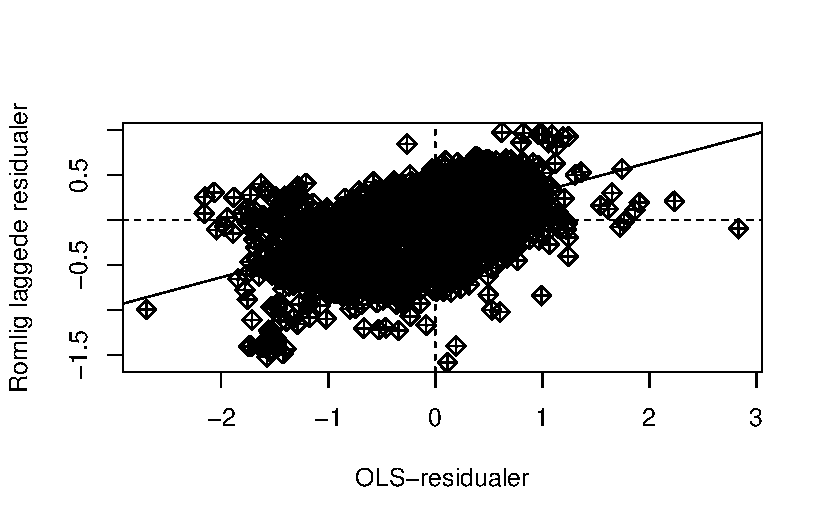
\includegraphics[keepaspectratio]{Arbeidskrav-MSB205_files/figure-pdf/fig-moran-ols-1.pdf}}

}

\caption{\label{fig-moran-ols}Moran-plott for OLS-residualene (k = 10).}

\end{figure}%

Tabell~\ref{tbl-moran-ols} viser at Moran's I for residualene fra
OLS-modellen er 0,365 med k = 3 og 0,319 med k = 10. Forventningen under
nullhypotesen er tilnærmet null (−0,001), og z-verdiene er henholdsvis
76,1 og 119,7. Nullhypotesen om ingen romlig autokorrelasjon forkastes
dermed klart for begge vektmatrisene.

Den positive helningen i Figur~\ref{fig-moran-ols} bekrefter dette.
Boliger der modellen undervurderer prisen, ligger gjerne nær andre
boliger der prisen også undervurderes. Det tyder på at det finnes
stedsspesifikke forhold som ikke fanges opp av forklaringsvariablene, og
vi går derfor videre med romlige regresjonsmodeller.

\subsection{Anselins tilnærming: Rao's
score-tester}\label{anselins-tilnuxe6rming-raos-score-tester}

Vi bruker to av de tre tilnærmingene til modellvalg som
Maslianskaia-Pautrel \& Baumont (2016) beskriver. Den første går fra det
spesifikke til det generelle og bygger på beslutningsregelen til Anselin
og kolleger (Maslianskaia-Pautrel \& Baumont, 2016, s. 934).

\[\text{SAR:} \quad y = \rho W y + X\beta + \varepsilon\]

\[\text{SEM:} \quad y = X\beta + u, \qquad u = \lambda W u + \varepsilon\]

I SAR-modellen påvirkes prisen på en bolig direkte av prisene på
naboboligene gjennom \(\rho Wy\). En intuitiv forklaring er at kjøpere
og eiendomsmeglere bruker nylige salg i nabolaget som referanse når de
vurderer prisen. SAR-modellen velges ofte i hedoniske studier nettopp
fordi «the market makes the prices» (Maslianskaia-Pautrel \& Baumont,
2016, s. 934). I SEM-modellen er den romlige avhengigheten knyttet til
feilleddet. Dette er aktuelt når det finnes uobserverte, romlig
korrelerte faktorer som påvirker prisene, men der naboprisene i seg selv
ikke har en egen effekt. Begge modellene nester OLS-modellen: dersom
\(\rho = 0\) eller \(\lambda = 0\), får vi tilbake den vanlige
OLS-modellen.

Valget mellom modellene gjøres ved hjelp av Rao's score-tester, også
kalt Lagrange multiplier-tester (LM-tester) (Maslianskaia-Pautrel \&
Baumont, 2016, s. 934). Fordelen med disse testene er at de bare krever
at OLS-modellen estimeres. \texttt{RSlag} tester nullhypotesen
\(\rho = 0\), og \texttt{RSerr} tester nullhypotesen \(\lambda = 0\).
Dersom bare én av testene er signifikant, velges den tilhørende
modellen. Dersom begge er signifikante, ser vi på de robuste variantene
\texttt{adjRSlag} og \texttt{adjRSerr}. Disse tester for én type
avhengighet samtidig som de tar hensyn til at den andre typen kan være
til stede. Modellen med den største robuste teststatistikken
foretrekkes. \texttt{SARMA} tester begge parametrene samtidig
(Maslianskaia-Pautrel \& Baumont, 2016, s. 934).

\begin{table}

\caption{\label{tbl-rstests}Rao's score-tester (LM) for
OLS-residualene.}

\centering{

\fontsize{12.0pt}{14.0pt}\selectfont
\begin{tabular*}{\linewidth}{@{\extracolsep{\fill}}lrrl}
\toprule
Test & Statistikk & df & p-verdi \\ 
\midrule\addlinespace[2.5pt]
\multicolumn{4}{l}{k = 3} \\[2.5pt] 
\midrule\addlinespace[2.5pt]
RSerr & 5 758,2 & 1 & < 0,001 \\ 
RSlag & 7 046,0 & 1 & < 0,001 \\ 
adjRSerr & 346,7 & 1 & < 0,001 \\ 
adjRSlag & 1 634,5 & 1 & < 0,001 \\ 
SARMA & 7 392,7 & 2 & < 0,001 \\ 
\midrule\addlinespace[2.5pt]
\multicolumn{4}{l}{k = 10} \\[2.5pt] 
\midrule\addlinespace[2.5pt]
RSerr & 14 186,3 & 1 & < 0,001 \\ 
RSlag & 11 959,7 & 1 & < 0,001 \\ 
adjRSerr & 4 344,7 & 1 & < 0,001 \\ 
adjRSlag & 2 118,1 & 1 & < 0,001 \\ 
SARMA & 16 304,4 & 2 & < 0,001 \\ 
\bottomrule
\end{tabular*}

}

\end{table}%

Tabell~\ref{tbl-rstests} viser at både RSlag og RSerr er svært
signifikante for begge vektmatrisene. Med et så stort datasett blir
nesten alle testene signifikante, og størrelsen på teststatistikkene er
derfor mer informativ enn p-verdiene. Vi må dessuten se på de robuste
testene. Her gir de to vektmatrisene ulike svar. Med k = 3 er den
robuste testen for lag-avhengighet (adjRSlag = 1 634,5) klart større enn
den for feilleddsavhengighet (adjRSerr = 346,7), noe som peker mot
SAR-modellen. Med k = 10 er forholdet motsatt: adjRSerr = 4 344.7 mot
adjRSlag = 2 118.1, noe som peker mot SEM-modellen.

Samtidig er begge de robuste testene signifikante for begge
vektmatrisene, og SARMA-testen er svært stor (7 392,7 og 16 304,4).
Dette tyder på at det finnes både lag- og feilleddsavhengighet i
dataene, og at verken SAR eller SEM alene er en fullgod spesifikasjon.
Anselins tilnærming gir oss dermed ikke en entydig konklusjon. Når
diagnostikken er uklar, kan vi sammenligne modellene direkte. Med k = 10
har SEM-modellen lavere AIC (5 072,0) enn SAR-modellen (5 204,3), noe
som støtter konklusjonen fra de robuste testene om at SEM er den beste
av de to. Uklarheten i resultatene er også en motivasjon for å bruke
LeSages tilnærming med nestede modeller.

\subsubsection{SAR-modellen og spatial
impacts}\label{sar-modellen-og-spatial-impacts}

I SAR-modellen kan ikke koeffisientene \(\beta\) tolkes direkte som
marginale effekter. Løser vi modellen for \(y\), får vi den reduserte
formen

\[y = (I - \rho W)^{-1} X\beta + (I - \rho W)^{-1} \varepsilon\]

Den partielle deriverte av \(y\) med hensyn på variabel \(x_r\) er
dermed en hel \(n \times n\)-matrise:

\[\frac{\partial y}{\partial x_r^{\top}} = (I - \rho W)^{-1} \beta_r = S_r(W)\]

Dette innebærer at en endring i en egenskap ved én bolig påvirker prisen
på boligen selv, prisene på naboboligene, prisene på naboenes naboer og
så videre. Effekten forplanter seg gjennom hele systemet, og spilloverne
er derfor globale (Maslianskaia-Pautrel \& Baumont, 2016, s. 927). Den
implisitte prisen er dermed mer enn den estimerte koeffisienten. Den
består av en direkte effekt, som inkluderer tilbakekoblingen via
naboene, og en indirekte effekt som spres til andre boliger (LeSage,
2014; Maslianskaia-Pautrel \& Baumont, 2016, s. 921--922). Disse
oppsummeres i direkte, indirekte og totale impacts, der den totale
effekten gir den implisitte prisen. Impactene forklares nærmere i
oppgave 8.

Fordi datasettet har over 25 000 observasjoner, er det svært tidkrevende
å beregne log-determinanten \(\ln|I - \rho W|\) eksakt. Modellen
estimeres derfor med \texttt{method\ =\ "MC"}, som tilnærmer
log-determinanten ved hjelp av Monte Carlo-simulering. Av samme grunn
beregnes impactene ved hjelp av sporene (traces) til potensene av \(W\).

\begin{table}

\caption{\label{tbl-sar-impacts}Impacts fra SAR-modellen (k = 10),
utvalgte variabler. p-verdier i parentes.}

\centering{

\fontsize{12.0pt}{14.0pt}\selectfont
\begin{tabular*}{\linewidth}{@{\extracolsep{\fill}}llll}
\toprule
Variabel & Direkte & Indirekte & Total \\ 
\midrule\addlinespace[2.5pt]
log\_TLA & 0,5136 (< 0,001) & 0,5536 (< 0,001) & 1,0672 (< 0,001) \\ 
age\_sold & 0,1802 (< 0,001) & 0,1942 (< 0,001) & 0,3744 (< 0,001) \\ 
log\_lot & 0,0728 (< 0,001) & 0,0785 (< 0,001) & 0,1513 (< 0,001) \\ 
dist\_CBD & −0,0014 (0,036) & −0,0015 (0,036) & −0,0029 (0,036) \\ 
pc\_inntekt\_1000 & −0,0014 (< 0,001) & −0,0015 (< 0,001) & −0,0028 (< 0,001) \\ 
andel\_svart & −0,3610 (< 0,001) & −0,3892 (< 0,001) & −0,7502 (< 0,001) \\ 
PM25 & 0,0875 (< 0,001) & 0,0944 (< 0,001) & 0,1819 (< 0,001) \\ 
\bottomrule
\end{tabular*}

}

\end{table}%

Den estimerte romlige autoregressive parameteren er \(\rho\) = 0,536, og
den er svært signifikant (z = 98,1). Prisen på en bolig henger altså
sterkt sammen med prisene på de ti nærmeste naboboligene. Fordi \(\rho\)
er såpass høy, blir den romlige multiplikatoren stor. Med en
radstandardisert vektmatrise er den totale effekten lik
\(\beta_r / (1 - \rho)\), altså omtrent 2,16 ganger koeffisienten.

Tabell~\ref{tbl-sar-impacts} viser impactene for et utvalg av
variablene. Impactene for boligareal og andelen svarte drøftes i oppgave
8. Avstand til CBD har en total effekt på −0,0029, som tilsvarer om lag
0,3 \% lavere pris per kilometer fra sentrum. Inntekt per innbygger har
en svakt negativ total effekt (−0,0028), i motsetning til den positive
effekten i SDEM. Fortegnet for denne variabelen er altså følsomt for
modellspesifikasjonen, noe som henger sammen med at den er sterkt
korrelert med de andre sosioøkonomiske variablene.

\subsection{LeSages tilnærming: lokalt eller globalt
fenomen?}\label{lesages-tilnuxe6rming-lokalt-eller-globalt-fenomen}

LeSage (2014) argumenterer for at valget av romlig modell bør begynne
med et teoretisk spørsmål: er spilloverne vi studerer lokale eller
globale? Ved globale spillovers forplanter en endring seg gjennom hele
systemet via naboenes naboer, slik som i SAR-modellen. Ved lokale
spillovers påvirker en endring bare de umiddelbare naboene, slik de er
definert i vektmatrisen, uten videre tilbakekobling. LeSage (2014)
hevder at de fleste problemstillinger i regionaløkonomi er av den lokale
typen. Maslianskaia-Pautrel \& Baumont (2016) tolker også den romlige
dimensjonen i hedoniske modeller som enten lokale eller globale
spillovers.

Vi mener at boligprisdannelse først og fremst er et \textbf{lokalt}
fenomen. En boligkjøper vurderer egenskapene ved boligen og de nærmeste
omgivelsene, som størrelsen og standarden på naboboligene,
inntektsnivået i nabolaget og miljøbelastningen der boligen ligger. Det
er lite sannsynlig at størrelsen på en bolig i Sylvania påvirker prisen
på en bolig i Toledo sentrum gjennom en lang kjede av naboer.

Dette er i tråd med Maslianskaia-Pautrel \& Baumont (2016), som påpeker
at hedonisk verdsetting er særlig egnet for miljøeksternaliteter med
lokale virkninger.

For lokale fenomener anbefaler LeSage (2014) å starte med Spatial Durbin
Error Model (SDEM). Dette tilsvarer tilnærmingen generelt-til-spesifikt
(Maslianskaia-Pautrel \& Baumont, 2016, s. 934):
\[\text{SDEM:} \quad y = X\beta + WX\theta + u, \qquad u = \lambda W u + \varepsilon\]

Her inngår både boligens egne egenskaper \(X\) og gjennomsnittet av
egenskapene til de \(k\) nærmeste naboene, \(WX\). I tillegg fanger
\(\lambda Wu\) opp uobserverte, romlig korrelerte faktorer. Fordi
modellen ikke inneholder \(Wy\), er impactene enkle å tolke: den direkte
effekten er \(\beta_r\), og den indirekte effekten er \(\theta_r\).

Vi inkluderer bare romlige lag for et utvalg av variablene, ved hjelp av
argumentet \texttt{Durbin\ =\ as.formula(\textasciitilde{}\ ...)}.
Tidsdummyene holdes utenfor, siden det ikke gir mening å tolke en
spillover fra salgsmåneden til naboboligene.

\subsection{Nestede modeller og likelihood
ratio-test}\label{nestede-modeller-og-likelihood-ratio-test}

SDEM-modellen nester tre enklere modeller, som vist i
Tabell~\ref{tbl-nesting}.

\begin{longtable}[]{@{}
  >{\raggedright\arraybackslash}p{(\linewidth - 2\tabcolsep) * \real{0.5000}}
  >{\raggedright\arraybackslash}p{(\linewidth - 2\tabcolsep) * \real{0.5000}}@{}}
\caption{Modeller som er nestet i
SDEM.}\label{tbl-nesting}\tabularnewline
\toprule\noalign{}
\begin{minipage}[b]{\linewidth}\raggedright
Restriksjon
\end{minipage} & \begin{minipage}[b]{\linewidth}\raggedright
Modell
\end{minipage} \\
\midrule\noalign{}
\endfirsthead
\toprule\noalign{}
\begin{minipage}[b]{\linewidth}\raggedright
Restriksjon
\end{minipage} & \begin{minipage}[b]{\linewidth}\raggedright
Modell
\end{minipage} \\
\midrule\noalign{}
\endhead
\bottomrule\noalign{}
\endlastfoot
\(\theta = 0\) & SEM:
\(y = X\beta + u, \ u = \lambda W u + \varepsilon\) \\
\(\lambda = 0\) & SLX: \(y = X\beta + WX\theta + \varepsilon\) \\
\(\theta = 0\) og \(\lambda = 0\) & OLS: \(y = X\beta + \varepsilon\) \\
\end{longtable}

SLX-modellen (spatial lag of X) inneholder bare lokale spillovers
gjennom \(WX\), og kan estimeres med OLS. SEM-modellen har bare romlig
avhengighet i feilleddet. Fordi modellene er nestet, kan vi teste
restriksjonene ved hjelp av en likelihood ratio-test (LeSage, 2014;
Maslianskaia-Pautrel \& Baumont, 2016, s. 934):

\[LR = -2 \left( \ln L_{\text{restriktert}} - \ln L_{\text{urestriktert}} \right) \sim \chi^2(m)\]

der \(m\) er antall restriksjoner. Nullhypotesen er at den restrikterte
modellen er tilstrekkelig. Forkastes nullhypotesen, foretrekkes den mer
generelle modellen. Vi tester SDEM mot SEM (\(\theta = 0\)), SDEM mot
SLX (\(\lambda = 0\)), og SEM og SLX mot OLS. SDEM- og SEM-modellene
estimeres med \texttt{method\ =\ "MC"}.

\begin{table}

\caption{\label{tbl-lr}Likelihood ratio-tester for de nestede
modellene.}

\centering{

\fontsize{12.0pt}{14.0pt}\selectfont
\begin{tabular*}{\linewidth}{@{\extracolsep{\fill}}lrrl}
\toprule
Test & LR & df & p-verdi \\ 
\midrule\addlinespace[2.5pt]
\multicolumn{4}{l}{k = 3} \\[2.5pt] 
\midrule\addlinespace[2.5pt]
SDEM vs SEM (θ = 0) & 764,2 & 5 & < 0,001 \\ 
SDEM vs SLX (λ = 0) & 5 090,0 & 1 & < 0,001 \\ 
SEM vs OLS (λ = 0) & 5 553,2 & 1 & < 0,001 \\ 
SLX vs OLS (θ = 0) & 1 227,4 & 5 & < 0,001 \\ 
\midrule\addlinespace[2.5pt]
\multicolumn{4}{l}{k = 10} \\[2.5pt] 
\midrule\addlinespace[2.5pt]
SDEM vs SEM (θ = 0) & 484,1 & 5 & < 0,001 \\ 
SDEM vs SLX (λ = 0) & 6 710,9 & 1 & < 0,001 \\ 
SEM vs OLS (λ = 0) & 7 744,9 & 1 & < 0,001 \\ 
SLX vs OLS (θ = 0) & 1 518,1 & 5 & < 0,001 \\ 
\bottomrule
\end{tabular*}

}

\end{table}%

\begin{table}

\caption{\label{tbl-aic-spatial}Log-likelihood og AIC for modellene.}

\centering{

\fontsize{12.0pt}{14.0pt}\selectfont
\begin{tabular*}{\linewidth}{@{\extracolsep{\fill}}lrr}
\toprule
Modell & logLik & AIC \\ 
\midrule\addlinespace[2.5pt]
\multicolumn{3}{l}{k = 3} \\[2.5pt] 
\midrule\addlinespace[2.5pt]
SDEM & -3 161,4 & 6 524,9 \\ 
SEM & -3 543,5 & 7 279,1 \\ 
SLX & -5 706,4 & 11 612,9 \\ 
OLS & -6 320,1 & 12 830,3 \\ 
\midrule\addlinespace[2.5pt]
\multicolumn{3}{l}{k = 10} \\[2.5pt] 
\midrule\addlinespace[2.5pt]
SDEM & -2 205,6 & 4 613,2 \\ 
SEM & -2 447,7 & 5 087,3 \\ 
SLX & -5 561,1 & 11 322,1 \\ 
OLS & -6 320,1 & 12 830,3 \\ 
\bottomrule
\end{tabular*}

}

\end{table}%

Tabell~\ref{tbl-lr} viser resultatene fra likelihood ratio-testene.
Testen av \(\theta = 0\) (SDEM mot SEM) gir LR = 760,6 med k = 3 og LR =
468,9 med k = 10, med 5 frihetsgrader. Testen av \(\lambda = 0\) (SDEM
mot SLX) gir LR = 5 083,3 og LR = 6 711 med én frihetsgrad. Begge
nullhypotesene forkastes klart for begge vektmatrisene. Verken de romlig
laggede forklaringsvariablene eller det romlige feilleddet kan dermed
utelates. Testene av SEM og SLX mot OLS er også klart signifikante, noe
som bekrefter at OLS-modellen ikke er tilstrekkelig.

Konklusjonen fra LeSages tilnærming er dermed at SDEM er den beste
modellen. Dette støttes av Tabell~\ref{tbl-aic-spatial}, der SDEM har
lavest AIC for begge vektmatrisene. Rangeringen er den samme for k = 3
og k = 10: SDEM, SEM, SLX og OLS. Videre har alle de romlige modellene
høyere log-likelihood med k = 10 enn med k = 3. For SDEM øker
log-likelihood fra −3 164,8 til −2 205,6. Vektmatrisen med ti naboer gir
dermed en bedre beskrivelse av den romlige strukturen, og vi bruker k =
10 i den videre tolkningen.

Det er verdt å merke seg at LR-testen av SEM mot OLS gir en mye større
teststatistikk (7 760,2 med k = 10) enn testen av SLX mot OLS (1 518,1).
Det romlige feilleddet forklarer altså langt mer av den romlige
avhengigheten enn de laggede forklaringsvariablene gjør. Dette tyder på
at mye av den romlige avhengigheten skyldes uobserverte nabolagsforhold,
og ikke spillovers fra naboboligenes målte egenskaper.

\begin{table}

\caption{\label{tbl-spatial-hus}Romlige modeller (k = 10), del 1:
konstantledd og huskarakteristika. Tidsdummyer inkludert, men ikke vist.
z- og t-verdier i parentes.}

\centering{

\fontsize{12.0pt}{14.0pt}\selectfont
\begin{tabular*}{\linewidth}{@{\extracolsep{\fill}}lccccc}
\toprule
  & OLS & SAR & SEM & SLX & SDEM \\ 
\midrule\addlinespace[2.5pt]
Konstantledd & 4,539*** & −0,102 & 5,514*** & 2,848*** & 3,638*** \\ 
 & (14,555) & (−0,380) & (6,503) & (9,158) & (4,647) \\ 
log\_TLA & 0,628*** & 0,495*** & 0,543*** & 0,587*** & 0,550*** \\ 
 & (56,509) & (52,150) & (56,275) & (51,977) & (57,120) \\ 
age\_sold & 0,208*** & 0,174*** & −0,311*** & 0,673*** & −0,256*** \\ 
 & (3,543) & (3,497) & (−4,622) & (11,376) & (−3,831) \\ 
age\_sold² & −0,919*** & −0,665*** & −0,059 & −1,210*** & −0,116 \\ 
 & (−8,615) & (−7,373) & (−0,506) & (−11,461) & (−1,002) \\ 
age\_sold³ & 0,037 & 0,043 & −0,144* & 0,135* & −0,134* \\ 
 & (0,625) & (0,854) & (−2,391) & (2,333) & (−2,246) \\ 
log\_lot & 0,109*** & 0,070*** & 0,121*** & 0,105*** & 0,119*** \\ 
 & (27,346) & (20,660) & (27,974) & (20,287) & (27,546) \\ 
rooms & −0,002 & −0,004 & −0,000 & −0,003 & −0,001 \\ 
 & (−0,514) & (−1,559) & (−0,011) & (−1,083) & (−0,325) \\ 
beds & 0,007 & 0,021*** & 0,017*** & 0,008 & 0,018*** \\ 
 & (1,455) & (5,403) & (4,465) & (1,851) & (4,703) \\ 
baths & 0,093*** & 0,041*** & 0,051*** & 0,078*** & 0,049*** \\ 
 & (15,354) & (8,035) & (9,883) & (13,163) & (9,395) \\ 
halfbaths & 0,066*** & 0,029*** & 0,037*** & 0,056*** & 0,036*** \\ 
 & (12,736) & (6,638) & (8,400) & (11,141) & (8,230) \\ 
Garasje: kjeller & 0,282*** & 0,210*** & 0,184*** & 0,284*** & 0,188*** \\ 
 & (7,820) & (6,874) & (6,238) & (8,108) & (6,376) \\ 
Garasje: tilbygd & 0,233*** & 0,159*** & 0,165*** & 0,200*** & 0,158*** \\ 
 & (29,265) & (23,592) & (24,031) & (25,748) & (23,055) \\ 
Garasje: frittstående & 0,242*** & 0,180*** & 0,151*** & 0,228*** & 0,151*** \\ 
 & (38,734) & (33,932) & (29,073) & (37,543) & (29,111) \\ 
Garasje: carport & 0,129*** & 0,102*** & 0,088*** & 0,117*** & 0,084*** \\ 
 & (5,890) & (5,522) & (4,858) & (5,466) & (4,641) \\ 
\bottomrule
\end{tabular*}
\begin{minipage}{\linewidth}
\vspace{.05em}
* p < 0.05, ** p < 0.01, *** p < 0.001\\
\end{minipage}

}

\end{table}%

\begin{table}

\caption{\label{tbl-spatial-omr}Romlige modeller (k = 10), del 2:
beliggenhet og områdevariabler. z- og t-verdier i parentes.}

\centering{

\fontsize{12.0pt}{14.0pt}\selectfont
\begin{tabular*}{\linewidth}{@{\extracolsep{\fill}}lccccc}
\toprule
  & OLS & SAR & SEM & SLX & SDEM \\ 
\midrule\addlinespace[2.5pt]
dist\_CBD & −0,004*** & −0,001* & −0,004 & −0,001 & −0,008*** \\ 
 & (−5,075) & (−2,020) & (−1,782) & (−1,746) & (−4,212) \\ 
pc\_inntekt\_1000 & 0,004*** & −0,001*** & 0,004*** & 0,001 & 0,001 \\ 
 & (9,895) & (−3,718) & (4,644) & (0,885) & (0,613) \\ 
andel\_svart & −0,658*** & −0,348*** & −0,638*** & 0,210 & 0,114 \\ 
 & (−51,256) & (−30,820) & (−18,245) & (1,958) & (1,199) \\ 
andel\_asiatisk & 0,984*** & 0,167 & 1,029*** & 0,871*** & 0,731* \\ 
 & (7,845) & (1,568) & (3,293) & (7,149) & (2,548) \\ 
andel\_ledige & −0,604*** & −0,078 & −0,989*** & −0,346*** & −0,638*** \\ 
 & (−12,592) & (−1,908) & (−9,018) & (−7,312) & (−6,163) \\ 
mwtt & −0,007*** & −0,003*** & −0,004* & −0,007*** & −0,007*** \\ 
 & (−7,566) & (−4,205) & (−1,980) & (−7,629) & (−3,342) \\ 
LOWINCPCT & −0,212*** & −0,042*** & −0,174*** & −0,127*** & −0,110*** \\ 
 & (−14,281) & (−3,346) & (−6,134) & (−8,692) & (−4,027) \\ 
LESSHSPCT & −0,943*** & −0,358*** & −0,779*** & −0,859*** & −0,714*** \\ 
 & (−30,627) & (−13,419) & (−13,164) & (−28,680) & (−12,686) \\ 
PTRAF & −0,000 & 0,000 & −0,000 & 0,000 & 0,000 \\ 
 & (−0,921) & (1,076) & (−0,159) & (0,907) & (0,419) \\ 
PRE1960PCT & −0,038*** & 0,108*** & −0,149*** & 0,161*** & 0,068** \\ 
 & (−3,602) & (11,814) & (−7,050) & (13,759) & (3,040) \\ 
PM25 & 0,106*** & 0,084*** & 0,072 & 0,163*** & 0,163* \\ 
 & (3,886) & (3,663) & (0,932) & (6,094) & (2,342) \\ 
\bottomrule
\end{tabular*}
\begin{minipage}{\linewidth}
\vspace{.05em}
* p < 0.05, ** p < 0.01, *** p < 0.001\\
\end{minipage}

}

\end{table}%

\begin{table}

\caption{\label{tbl-spatial-romlig}Romlige modeller (k = 10), del 3:
romlige lag, romlige parametere og modelltilpasning. z-verdier i
parentes.}

\centering{

\fontsize{12.0pt}{14.0pt}\selectfont
\begin{tabular*}{\linewidth}{@{\extracolsep{\fill}}lcccc}
\toprule
  & SAR & SEM & SLX & SDEM \\ 
\midrule\addlinespace[2.5pt]
W · log\_TLA &  &  & 0,219*** & 0,129*** \\ 
 &  &  & (17,094) & (6,327) \\ 
W · age\_sold &  &  & −0,637*** & −0,504*** \\ 
 &  &  & (−32,672) & (−16,497) \\ 
W · log\_lot &  &  & −0,014 & 0,011 \\ 
 &  &  & (−1,942) & (0,942) \\ 
W · pc\_inntekt\_1000 &  &  & 0,001 & 0,003 \\ 
 &  &  & (0,567) & (1,767) \\ 
W · andel\_svart &  &  & −0,912*** & −0,869*** \\ 
 &  &  & (−8,460) & (−8,815) \\ 
ρ & 0,536*** &  &  &  \\ 
 & (98,081) &  &  &  \\ 
λ &  & 0,727*** &  & 0,693*** \\ 
{} & {} & {(118,981)} & {} & {(108,062)} \\ 
Antall obs. & 25 213 & 25 213 & 25 213 & 25 213 \\ 
AIC & 5 204,3 & 5 087,3 & 11 322,1 & 4 613,2 \\ 
Log-likelihood &  &  & −5 561,1 &  \\ 
\bottomrule
\end{tabular*}
\begin{minipage}{\linewidth}
\vspace{.05em}
* p < 0.05, ** p < 0.01, *** p < 0.001\\
\end{minipage}

}

\end{table}%

Tabell~\ref{tbl-spatial-romlig} viser at de romlige parameterne er store
og svært signifikante: \(\rho\) = 0,536 i SAR-modellen, og \(\lambda\) =
0,729 i SEM-modellen og 0,693 i SDEM-modellen.

Koeffisientene for huskarakteristikaene er stabile på tvers av modellene
og har forventet fortegn (Tabell~\ref{tbl-spatial-hus}). Boligareal,
tomtestørrelse, antall bad og halvbad og garasje har alle positive og
signifikante effekter. For eksempel gir en frittstående garasje omtrent
16 \% høyere pris i SDEM-modellen (exp(0,151) − 1), sammenlignet med en
bolig uten garasje.

Avstand til CBD har negativt fortegn i alle de romlige modellene. I
SDEM-modellen er koeffisienten −0,008, noe som betyr at prisen faller
med omtrent 0,8 \% per kilometer lenger fra sentrum, alt annet likt.
Dette står i kontrast til den positive koeffisienten i modell 2 (0,013).
Forskjellen skyldes trolig at modell 2 bare kontrollerte for boligareal.
Boliger i forstedene har større tomter, er nyere og har oftere garasje,
og når vi kontrollerer for disse egenskapene, får vi det fortegnet den
monosentriske bymodellen forutsier.

Flere av områdevariablene endrer fortegn eller signifikans mellom
modellene. Andelen boliger bygget før 1960 (PRE1960PCT) er negativ i OLS
og SEM, men positiv i SAR, SLX og SDEM. PM2,5 er positiv i flere av
modellene. Dette tyder på at områdevariablene, som er målt på tract-
eller blokknivå, er sterkt korrelert med hverandre og med den romlige
strukturen i dataene. Koeffisientene for disse variablene bør derfor
tolkes med forsiktighet.

\begin{table}

\caption{\label{tbl-sdem-slx-impacts}Direkte, indirekte og totale
impacts fra SDEM og SLX (k = 10). z-verdier i parentes.}

\centering{

\fontsize{12.0pt}{14.0pt}\selectfont
\begin{tabular*}{\linewidth}{@{\extracolsep{\fill}}llll}
\toprule
Variabel & Direkte & Indirekte & Total \\ 
\midrule\addlinespace[2.5pt]
\multicolumn{4}{l}{SDEM} \\[2.5pt] 
\midrule\addlinespace[2.5pt]
log\_TLA & 0,550 (57,0) & 0,129 (6,3) & 0,679 (29,2) \\ 
age\_sold & −0,256 (−3,8) & −0,504 (−16,5) & −0,761 (−10,3) \\ 
log\_lot & 0,119 (27,5) & 0,011 (0,9) & 0,129 (11,2) \\ 
pc\_inntekt\_1000 & 0,001 (0,6) & 0,003 (1,8) & 0,004 (3,8) \\ 
andel\_svart & 0,114 (1,2) & −0,869 (−8,8) & −0,755 (−22,8) \\ 
\midrule\addlinespace[2.5pt]
\multicolumn{4}{l}{SLX} \\[2.5pt] 
\midrule\addlinespace[2.5pt]
log\_TLA & 0,587 (52,0) & 0,219 (17,1) & 0,805 (55,8) \\ 
age\_sold & 0,673 (11,4) & −0,637 (−32,7) & 0,036 (0,6) \\ 
log\_lot & 0,105 (20,3) & −0,014 (−1,9) & 0,091 (16,4) \\ 
pc\_inntekt\_1000 & 0,001 (0,9) & 0,001 (0,6) & 0,002 (5,7) \\ 
andel\_svart & 0,210 (2,0) & −0,912 (−8,5) & −0,703 (−55,2) \\ 
\bottomrule
\end{tabular*}

}

\end{table}%

Tabell~\ref{tbl-sdem-slx-impacts} viser direkte, indirekte og totale
impacts fra SDEM- og SLX-modellene for variablene som inngår med romlige
lag. Impactene for boligareal og andelen svarte drøftes i oppgave 8. Her
ser vi på de øvrige variablene.

\textbf{Tomtestørrelse og alder.} Tomtestørrelsen hos naboene har ingen
signifikant effekt (z = 0,9). Kjøpere legger altså vekt på sin egen
tomt, men ikke på hvor store tomter naboene har. Alderen på naboboligene
har derimot en sterk negativ effekt (−0,504, z = −16,5). Boliger i
nabolag med eldre boligmasse har dermed lavere priser, uavhengig av
boligens egen alder. Den direkte effekten av alder må tolkes sammen med
andre- og tredjegradsleddene, og er derfor vanskeligere å tolke direkte.

\textbf{Inntekt per innbygger.} For inntekt per innbygger ser vi det
samme mønsteret som for andelen svarte. Verken den direkte effekten
(0,0009, z = 0,6) eller den indirekte effekten (0,0030, z = 1,8) er
signifikant på 5 \%-nivå hver for seg. Den totale effekten (0,0039) er
derimot klart signifikant (z = 3,8). Det betyr at 1 000 dollar høyere
inntekt per innbygger i nabolaget er forbundet med omtrent 0,4 \% høyere
boligpris, alt annet likt. At standardfeilen for den totale effekten er
mye mindre enn for de to delene, er et typisk tegn på
multikollinearitet: modellen kan anslå den samlede effekten presist, men
ikke fordele den mellom boligens egen tract og naboenes. Effekten er
moderat, noe som henger sammen med at modellen også inneholder andre
sterkt korrelerte sosioøkonomiske variabler, som andelen med lav inntekt
(−0,110) og andelen uten videregående utdanning (−0,714).

\textbf{Sammenligning med SLX.} Den indirekte effekten av boligareal er
0,219 i SLX, men bare 0,129 i SDEM. Den totale effekten faller
tilsvarende fra 0,805 til 0,679. Forskjellen skyldes at SLX-modellen
ikke har et romlig feilledd. Uobserverte nabolagsforhold, som generell
attraktivitet eller kvaliteten på skoler, vil da delvis fanges opp av de
laggede forklaringsvariablene. Store boliger ligger gjerne i attraktive
nabolag, og i SLX tilskrives noe av nabolagets attraktivitet
naboboligenes størrelse. Når \(\lambda Wu\) tar opp denne avhengigheten
i SDEM, blir spillover-effekten mindre. Også for alder gir modellene
ulike svar: i SLX er den direkte effekten positiv (0,673) og den totale
effekten ikke signifikant (z = 0,6), mens både den direkte og den totale
effekten er negativ og signifikant i SDEM. Dette illustrerer hvorfor det
er viktig å kontrollere for romlig avhengighet i feilleddet. Ellers
risikerer vi å overvurdere de lokale spillovereffektene.

\subsection{Hvor godt fjerner modellene de romlige
effektene?}\label{hvor-godt-fjerner-modellene-de-romlige-effektene}

Til slutt undersøker vi hvor godt de ulike modellene fjerner den romlige
avhengigheten i residualene, ved hjelp av Moran-plott og Moran's I for
residualene fra OLS, SLX, SAR, SEM og SDEM med \(k = 10\).

\begin{figure}[H]

\centering{

\pandocbounded{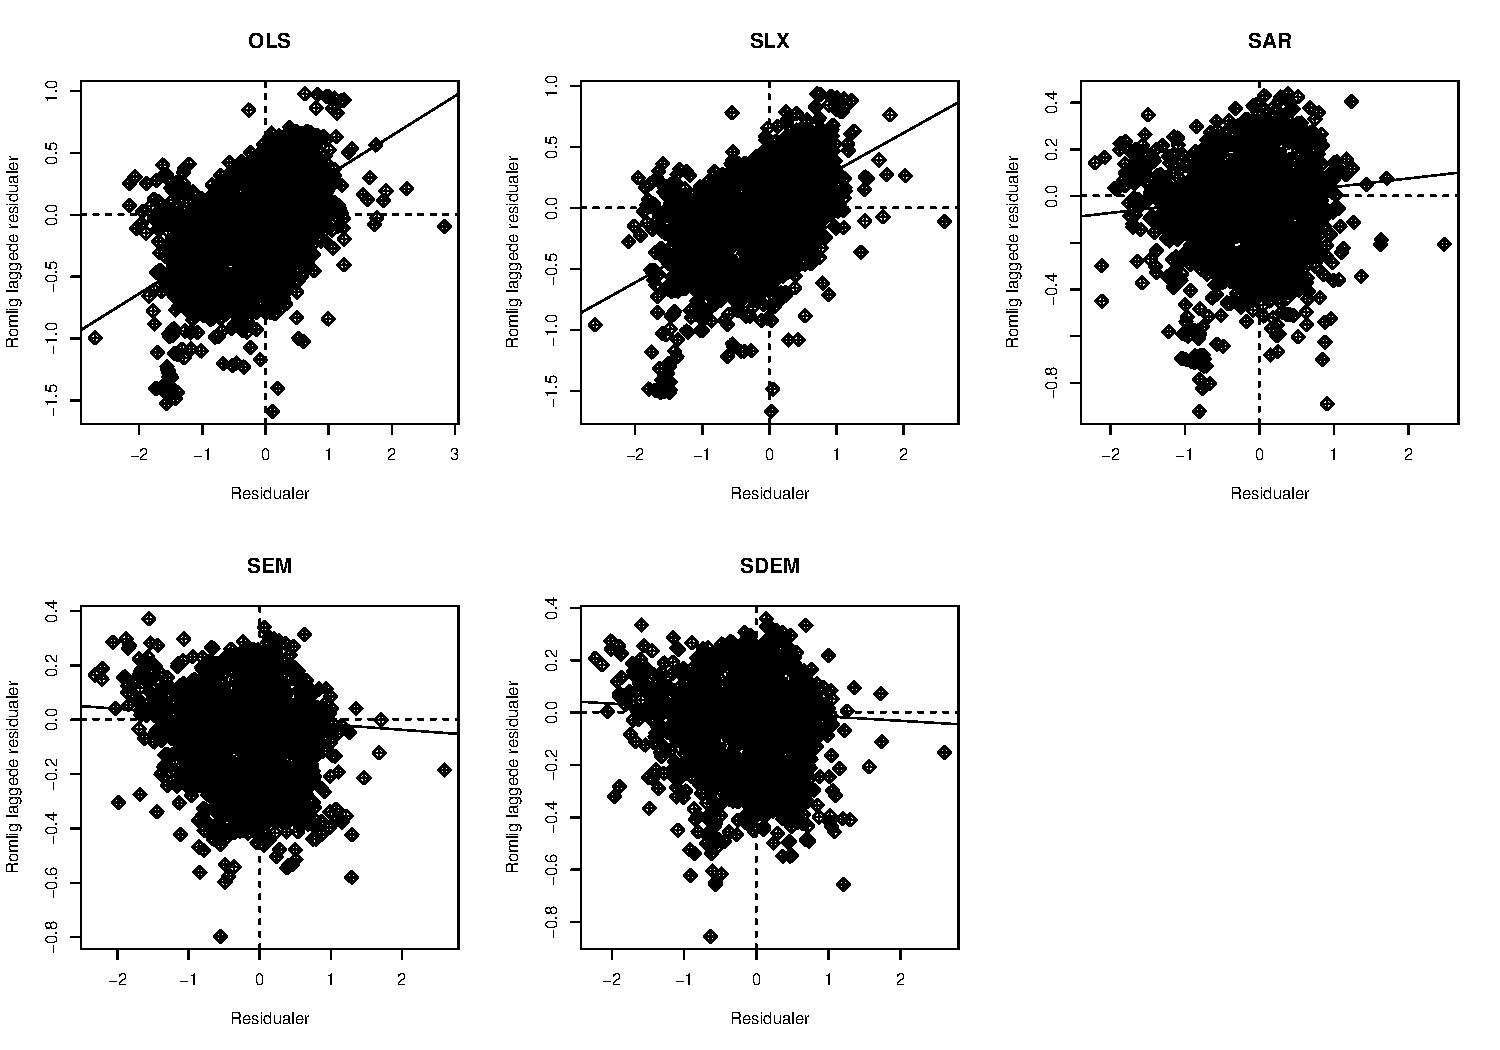
\includegraphics[keepaspectratio]{Arbeidskrav-MSB205_files/figure-pdf/fig-moran-models-1.pdf}}

}

\caption{\label{fig-moran-models}Moran-plott for residualene fra de
ulike modellene (k = 10).}

\end{figure}%

\begin{table}

\caption{\label{tbl-moran-models}Moran's I for residualene fra hver
modell (k = 10).}

\centering{

\fontsize{12.0pt}{14.0pt}\selectfont
\begin{tabular*}{\linewidth}{@{\extracolsep{\fill}}lrl}
\toprule
Modell & Moran's I & p-verdi \\ 
\midrule\addlinespace[2.5pt]
OLS & 0,319 & < 0,001 \\ 
SLX & 0,306 & < 0,001 \\ 
SAR & 0,037 & < 0,001 \\ 
SEM & -0,019 & 1,000 \\ 
SDEM & -0,017 & 1,000 \\ 
\bottomrule
\end{tabular*}

}

\end{table}%

Figur~\ref{fig-moran-models} og Tabell~\ref{tbl-moran-models} viser at
det er tydelige forskjeller mellom modellene.

Residualene fra OLS- og SLX-modellene har fortsatt en klar positiv
helning, med Moran's I på henholdsvis 0,319 og 0,306. At de romlig
laggede forklaringsvariablene i SLX bare reduserer Moran's I marginalt,
viser at naboboligenes målte egenskaper i liten grad forklarer den
romlige avhengigheten. Mesteparten av avhengigheten skyldes forhold som
ikke er målt i modellen.

SAR-modellen fjerner det meste av autokorrelasjonen, og Moran's I faller
til 0,037. Verdien er likevel fortsatt signifikant positiv (p
\textless{} 0,001), og plottet viser en svak positiv helning. Det
romlige laget i den avhengige variabelen fanger altså opp mye, men ikke
all, romlig avhengighet.

For SEM- og SDEM-modellene er punktskyen tilnærmet flat, og Moran's I er
svakt negativ (−0,020 og −0,017). Det er ingen gjenværende positiv
romlig autokorrelasjon i residualene fra disse modellene. Dette er som
forventet, siden det romlige feilleddet \(\lambda Wu\) nettopp er ment å
fange opp romlig korrelerte uobserverte faktorer. Den svakt negative
verdien kan tyde på at feilleddsmodellene i noen grad overkorrigerer,
men verdiene er så små at de har liten praktisk betydning.

\subsection{Oppsummering av
modellvalget}\label{oppsummering-av-modellvalget}

Anselins LM-tester ga ikke et entydig svar, mens LeSages nestede
tilnærming klart pekte på SDEM for begge vektmatrisene. Rangeringen av
modellene er den samme for k = 3 og k = 10, men k = 10 gir høyest
log-likelihood, og Moran-plottene viser at SDEM fjerner den positive
romlige autokorrelasjonen i residualene. Vi bruker derfor SDEM-modellen
med k = 10 som vår foretrukne modell. Forskjellen mellom de to
tilnærmingene drøftes i oppgave 8.

\section{Oppgave 8 Diskusjon av
resultatene}\label{oppgave-8-diskusjon-av-resultatene}

\subsection{Økonomisk tolkning av den hedoniske
prismodellen}\label{uxf8konomisk-tolkning-av-den-hedoniske-prismodellen}

Den hedoniske prismodellen viser at prisen på et differensiert gode kan
forklares ut fra egenskapene til godet (Bishop et al., 2020, s. 262;
Maslianskaia-Pautrel \& Baumont, 2016, s. 923). En bolig består av en
pakke med egenskaper: egenskaper ved selve boligen (H), som areal, alder
og antall bad, og egenskaper ved beliggenheten (X), som avstand til
sentrum, nabolagets sosioøkonomiske sammensetning og miljøforhold
(Maslianskaia-Pautrel \& Baumont, 2016, s. 923--924). Den hedoniske
prisfunksjonen kan dermed skrives som

\[P = f(H, X_{env}, X_{other})\]

Den hedoniske prisfunksjonen er verken en etterspørselsfunksjon eller en
tilbudsfunksjon. Den er en likevektsrelasjon som oppstår gjennom
samspillet mellom kjøpere og selgere i boligmarkedet (Bishop et al.,
2020, s. 262; Maslianskaia-Pautrel \& Baumont, 2016, s. 923). I likevekt
kan ingen husholdninger øke nytten ved å flytte. Den deriverte av
prisfunksjonen med hensyn på en egenskap kan da tolkes som den
\emph{implisitte prisen} på egenskapen:

\[MWTP_k = \frac{\partial P}{\partial x_k}\]

Den implisitte prisen tilsvarer kjøpernes marginale betalingsvillighet
(MWTP) for egenskapen (Bishop et al., 2020, s. 261--263;
Maslianskaia-Pautrel \& Baumont, 2016, s. 924). Tolkningen forutsetter
at kjøperne er fullt informert, kan flytte fritt og kan velge
kontinuerlige mengder av hver egenskap (Bishop et al., 2020, s. 262).

I vår modell er den avhengige variabelen logaritmen av salgsprisen.
Koeffisientene tolkes derfor som prosentvise endringer i prisen. For
logaritmerte forklaringsvariabler, som boligareal, er koeffisientene
elastisiteter. For dummyvariabler og variabler målt i nivå gir
\(100 \cdot (\exp(\beta) - 1)\) den eksakte prosentvise endringen.
Tidsdummyene fanger opp endringer i det generelle prisnivået i perioden
1993--1998. Dette er viktig fordi prisfunksjonen og de implisitte
prisene kan endre seg over tid (Bishop et al., 2020, s. 264).

\subsection{Hvorfor trenger vi romlige
regresjonsmodeller?}\label{hvorfor-trenger-vi-romlige-regresjonsmodeller}

Det er tre hovedgrunner til at vi trenger romlige regresjonsmodeller i
en hedonisk analyse av boligpriser.

\textbf{For det første er boligpriser og egenskapene deres romlig
avhengige.} Like priser observeres oftere nær hverandre enn om prisene
var tilfeldig fordelt, og forklaringsvariablene, som miljøforhold og
nabolagskvalitet, er også romlig avhengige (Maslianskaia-Pautrel \&
Baumont, 2016, s. 924). Dette ser vi tydelig i våre data. EDA-en i
Seksjon~\ref{sec-eda} viste klare klynger av dyre og billige boliger, og
Moran's I for residualene fra OLS-modellen er 0,319 med ti naboer
(Tabell~\ref{tbl-moran-ols}). Mange egenskaper ved nabolaget er
vanskelige å måle og havner derfor i feilleddet. Når de er romlig
korrelerte, blir også residualene romlig korrelerte (Bishop et al.,
2020, s. 270).

\textbf{For det andre gir OLS dårligere estimater når det finnes romlig
avhengighet.} Hvis den romlige avhengigheten ligger i feilleddet, er
OLS-estimatene ineffisiente og standardfeilene upålitelige. Hvis prisene
påvirker hverandre direkte, slik som i SAR-modellen, blir OLS-estimatene
også forventningsskjeve (Maslianskaia-Pautrel \& Baumont, 2016, s. 938).

\textbf{For det tredje kan den implisitte prisen bli feiltolket.}
Maslianskaia-Pautrel \& Baumont (2016) understreker at romlige
prosesser, i form av spredning og multiplikatoreffekter, gjør at den
implisitte prisen ikke bare er den estimerte koeffisienten. Den består
av en direkte effekt og en indirekte effekt som kommer fra naboene. Hvis
vi ignorerer dette, risikerer vi å feilberegne betalingsvilligheten for
egenskaper ved boligen og nabolaget (Maslianskaia-Pautrel \& Baumont,
2016, s. 941--924).

Det finnes også teoretiske grunner til å forvente romlige effekter i
boligmarkedet. Kjøpere, selgere og eiendomsmeglere bruker salg i
nabolaget som referanse for prisen, slik at «the market makes the
prices» (Maslianskaia-Pautrel \& Baumont, 2016, s. 924). I tillegg
kapitaliseres romlig variasjon i lokale goder og ulemper i boligprisene
(Bishop et al., 2020, s. 260), og miljøeksternaliteter har ofte lokale
virkninger (Maslianskaia-Pautrel \& Baumont, 2016, s. 924).

\subsection{Tre metoder for å velge
modellspesifikasjon}\label{tre-metoder-for-uxe5-velge-modellspesifikasjon}

Maslianskaia-Pautrel \& Baumont (2016) beskriver tre tilnærminger til å
velge den mest hensiktsmessige romlige modellen:

\begin{enumerate}
\def\labelenumi{\arabic{enumi}.}
\tightlist
\item
  \textbf{Spesifikt-til-generelt.} Vi starter med en ikke-romlig modell,
  som OLS, og tester om en mer generell romlig modell er bedre. Valget
  mellom SAR og SEM gjøres ved hjelp av Lagrange multiplier-testene
  LMERR og LMLAG og de robuste variantene av dem. Denne tilnærmingen har
  tradisjonelt vært mest brukt.
\item
  \textbf{Generelt-til-spesifikt.} Vi starter med den mest generelle
  modellen, SDM eller SDEM, og tester trinn for trinn om restriksjoner
  på de romlige parameterne (\(\rho\), \(\lambda\) eller \(\theta\)) kan
  aksepteres. Testene gjøres med likelihood ratio-tester. Ifølge
  forfatterne anbefales denne tilnærmingen i økende grad.
\item
  \textbf{«Story».} Modellen velges ut fra teori eller forhåndskunnskap
  om fenomenet. SAR-modellen velges for eksempel ofte i hedoniske
  studier fordi «the market makes the prices», SLX-modellen fordi den
  fanger opp eksternaliteter fra nabolaget, og SEM-modellen som en
  korreksjon for utelatte variabler og feilspesifikasjon.
\end{enumerate}

Forfatterne påpeker at det ikke finnes noen etablert enighet om hvilken
tilnærming som er best (Maslianskaia-Pautrel \& Baumont, 2016, s. 934).

I denne oppgaven har vi brukt de to første tilnærmingene. Anselins
metode med Rao's score-tester (Tabell~\ref{tbl-rstests}) er tilnærmingen
spesifikt-til-generelt. Den ga ikke et entydig svar: med k = 3 pekte de
robuste testene mot SAR, og med k = 10 mot SEM. Metiden til LeSage
(2014) med nestede modeller og LR-tester (Tabell~\ref{tbl-lr}) er
tilnærmingen generelt-til-spesifikt, med SDEM som utgangspunkt. Den ga
en klar konklusjon om at SDEM er den beste modellen. Vi har også trukket
inn elementer fra den tredje tilnærmingen. Valget av SDEM framfor SDM
som utgangspunkt bygger på en teoretisk vurdering av at
boligprisdannelse er et lokalt og ikke et globalt fenomen. At metodene
gir ulike svar, henger sammen med at Anselins tester bare velger mellom
SAR og SEM ut fra OLS-residualene, uten å vurdere romlige lag i
forklaringsvariablene. LeSages tilnærming starter derimot i den mest
generelle lokale modellen og tester restriksjonene.

\subsection{Tolkning av
koeffisientene}\label{tolkning-av-koeffisientene}

Vi ser nærmere på to variabler: boligareal (\texttt{log\_TLA}) og
andelen svarte i census tracten (\texttt{andel\_svart}).
Tabell~\ref{tbl-diskusjon} oppsummerer estimatene fra de ulike modellene
med k = 10. For SAR, SLX og SDEM viser tabellen impactene, siden det er
disse som gir den implisitte prisen.

\begin{longtable}[]{@{}llll@{}}
\caption{Estimerte effekter av boligareal og andel svarte i de ulike
modellene (k = 10). t- eller z-verdier i parentes. Alle effektene i
SAR-modellen er signifikante på 0,1
\%-nivå.}\label{tbl-diskusjon}\tabularnewline
\toprule\noalign{}
Modell & Effekt & Boligareal (log) & Andel svarte \\
\midrule\noalign{}
\endfirsthead
\toprule\noalign{}
Modell & Effekt & Boligareal (log) & Andel svarte \\
\midrule\noalign{}
\endhead
\bottomrule\noalign{}
\endlastfoot
OLS & Koeffisient & 0,628 (56,5) & −0,658 (−51,3) \\
SEM & Koeffisient & 0,543 (56,3) & −0,638 (−18,2) \\
SAR & Direkte & 0,514 & −0,361 \\
& Indirekte & 0,554 & −0,389 \\
& Total & 1,067 & −0,750 \\
SLX & Direkte & 0,587 (52,0) & 0,210 (2,0) \\
& Indirekte & 0,219 (17,1) & −0,912 (−8,5) \\
& Total & 0,805 (55,8) & −0,703 (−55,2) \\
SDEM & Direkte & 0,550 (57,1) & 0,114 (1,2) \\
& Indirekte & 0,129 (6,3) & −0,869 (−8,8) \\
& Total & 0,679 (29,2) & −0,755 (−22,7) \\
\end{longtable}

\textbf{I OLS- og SEM-modellene} tolkes koeffisientene direkte.
Boligareal inngår logaritmert, så koeffisienten er en elastisitet: i
OLS-modellen gir 1 \% større boligareal 0,63 \% høyere pris, alt annet
likt. Andelen svarte er målt som en andel mellom 0 og 1. En økning på 10
prosentpoeng gir derfor en endring i prisen på
\(\exp(-0{,}0658) - 1 \approx -6{,}4\) \% i OLS og \(-6{,}2\) \% i SEM.
Fordi SEM-modellen bare har romlig avhengighet i feilleddet, er
koeffisientene fortsatt de implisitte prisene (Maslianskaia-Pautrel \&
Baumont, 2016, s. 927).

\textbf{I SAR-modellen} kan koeffisientene ikke tolkes direkte, fordi en
endring i én bolig forplanter seg via \(\rho W y\) til hele systemet. Vi
må derfor bruke impactene, som diskuteres nærmere nedenfor.

\textbf{I SLX- og SDEM-modellene} er den direkte effekten lik
koeffisienten for variabelen selv (\(\beta\)). Den indirekte effekten er
lik koeffisienten for det romlige laget (\(\theta\)), og måler hvordan
prisen endres når gjennomsnittet av variabelen blant de ti nærmeste
naboene endres. Den implisitte prisen er summen av de to
(Maslianskaia-Pautrel \& Baumont, 2016, s. 938). I SDEM-modellen gir 1
\% større boligareal 0,55 \% høyere pris for boligen selv. Om
gjennomsnittsarealet blant naboboligene også øker med 1 \%, øker prisen
med ytterligere 0,13 \%, til sammen 0,68 \%. Med en gjennomsnittspris på
om lag 79 000 dollar tilsvarer den totale effekten omtrent 540 dollar.

\subsection{Er koeffisientene signifikante og
rimelige?}\label{er-koeffisientene-signifikante-og-rimelige}

\textbf{Boligareal} er positiv og signifikant på 0,1 \%-nivå i alle
modellene. Fortegnet er som forventet: større boliger er dyrere.
Elastisiteten ligger mellom 0,54 og 0,63 for den direkte effekten. Det
betyr at prisen øker mindre enn proporsjonalt med arealet, noe som er
rimelig, fordi den marginale verdien av ekstra areal er avtakende. Det
er også verdt å merke seg hvordan koeffisienten endrer seg når vi
kontrollerer for flere forhold. I modell 1, der boligareal er den eneste
huskarakteristikken, er elastisiteten 1,27. Den faller til 0,80 i modell
2 og til 0,63 i OLS-modellen i oppgave 7, der vi kontrollerer for flere
huskarakteristika. Den faller videre til 0,54--0,55 i SEM og SDEM, der
det romlige feilleddet fanger opp uobserverte nabolagsforhold. Dette
tyder på at de enklere modellene overvurderer effekten av boligareal,
fordi store boliger gjerne har andre attraktive egenskaper og ligger i
attraktive nabolag. Det er et eksempel på skjevhet fra utelatte
variabler (Bishop et al., 2020, s. 270).

Den totale effekten av boligareal er derimot klart større i SAR-modellen
(1,067) enn i de andre modellene. En total elastisitet over 1 virker
urimelig høy, og skyldes den globale multiplikatoren i SAR-modellen. I
SDEM, som er vår foretrukne modell, er den totale effekten 0,68. Det er
et mer troverdig anslag på den implisitte prisen.

\textbf{Andelen svarte} er negativ og signifikant i OLS, SEM og SAR. I
SLX og SDEM er det bare den indirekte og den totale effekten som er
klart signifikante. Den direkte effekten er ikke signifikant i SDEM og
svakt positiv i SLX (z = 2,0). Dette er ikke et uttrykk for at den
direkte effekten er null eller positiv. Det skyldes at X og WX er nesten
perfekt korrelert for denne variabelen (0,996), slik at modellen ikke
kan skille de to effektene. Den totale effekten er derimot svært stabil
på tvers av modellene: mellom −0,64 og −0,76. Det tilsvarer omtrent 6--7
\% lavere boligpris når andelen svarte i nabolaget øker med 10
prosentpoeng.

Fortegnet er i tråd med EDA-en, som viste at de billigste boligene
ligger i sentrumsnære bydeler. Det er likevel viktig å understreke at
denne effekten ikke kan tolkes som en kausal effekt av etnisitet eller
som kjøpernes betalingsvillighet for nabolagets etniske sammensetning.
Variabelen fanger trolig opp andre forhold som er korrelert med
befolkningssammensetningen, som historisk segregering, skolekvalitet og
andre sosioøkonomiske forskjeller (Bishop et al., 2020, s. 270).
Forutsetningen om at kjøperne kan flytte fritt (Bishop et al., 2020, s.
262) holder heller ikke nødvendigvis i et marked preget av segregering.

Til slutt bør det nevnes at alle variablene blir signifikante med over
25 000 observasjoner, så størrelsen og fortegnet er mer informative enn
p-verdiene. Breusch-Pagan-testen i oppgave 5 viste dessuten at
feilleddene er heteroskedastiske. Standardfeilene i de romlige modellene
er ikke korrigert for dette, og t- og z-verdiene bør derfor tolkes med
en viss forsiktighet.

\subsection{Spatial impacts i
SAR-modellen}\label{spatial-impacts-i-sar-modellen}

I SAR-modellen inngår prisene på naboboligene som en forklaringsvariabel
gjennom \(\rho W y\). Når en egenskap ved én bolig endres, påvirkes
prisen på boligen selv, men også prisene på naboboligene, og deretter
prisene på naboenes naboer og så videre. Den implisitte prisen består
derfor av mer enn koeffisienten. Den kombinerer en tilbakekoblingseffekt
(«feedback effect») og en spredningseffekt («propagation effect»)
(Maslianskaia-Pautrel \& Baumont, 2016, s. 921). \emph{Spatial impacts}
er målene vi bruker for å oppsummere disse effektene (LeSage, 2014;
Maslianskaia-Pautrel \& Baumont, 2016, s. 921--922):

\begin{itemize}
\tightlist
\item
  \textbf{Den direkte effekten} måler hvor mye prisen på en bolig endres
  når en egenskap ved boligen selv endres, inkludert tilbakekoblingen:
  endringen påvirker naboene, som igjen påvirker den opprinnelige
  boligen.
\item
  \textbf{Den indirekte effekten} måler hvor mye prisen på en bolig
  endres når egenskapen endres hos alle de andre boligene. Dette er
  spillover-effekten.
\item
  \textbf{Den totale effekten} er summen av de to, og gir den implisitte
  prisen for egenskapen (Maslianskaia-Pautrel \& Baumont, 2016, s. 938)
\end{itemize}

\textbf{Boligareal.} Koeffisienten i SAR-modellen er 0,495, mens den
direkte effekten er 0,514. Differansen på 0,019 er tilbakekoblingen: når
en bolig blir større og dyrere, øker prisene på naboboligene noe, og det
gir igjen et lite tillegg til prisen på den opprinnelige boligen. Den
indirekte effekten er 0,554. Den viser at prisen på en bolig øker med om
lag 0,55 \% hvis alle de andre boligene blir 1 \% større. Den økonomiske
mekanismen er at kjøpere og meglere bruker salgsprisene på nabolagets
boliger som referanse. Større boliger i nabolaget gir høyere
referansepriser, og dette spres videre i markedet. Den totale effekten
er 1,067. Dette er den implisitte prisen ifølge SAR-modellen: hvis alle
boligene ble 1 \% større, ville prisen på en gitt bolig øke med om lag
1,07 \%. Ved en gjennomsnittspris på 79 000 dollar tilsvarer det om lag
840 dollar.

\textbf{Andelen svarte.} Koeffisienten er −0,348, mens den direkte
effekten er −0,361. Tilbakekoblingen er dermed −0,013. Den indirekte
effekten er −0,389, og den totale effekten −0,750. Det betyr at en
økning i andelen svarte på 10 prosentpoeng i hele området er forbundet
med om lag 7,2 \% lavere boligpris. Litt over halvparten av effekten
kommer gjennom spredning via prisene på naboboligene.

Et viktig poeng er at forholdet mellom den indirekte og den direkte
effekten er det samme, omtrent 1,08, for alle variablene i SAR-modellen
(Tabell~\ref{tbl-sar-impacts}). Dette er ikke et empirisk resultat, men
en følge av at alle spillovers styres av den samme parameteren \(\rho\).
SDEM-modellen har ikke denne begrensningen. Der er den indirekte
effekten av boligareal bare 0,129, eller om lag en fjerdedel av den
direkte effekten, mens den indirekte effekten av andelen svarte er
større enn den direkte. Siden LR-testene og AIC viser at SDEM er den
beste modellen, mener vi at de totale effektene fra SDEM gir de mest
troverdige anslagene på de implisitte prisene. For boligareal er dette
0,68 og for andelen svarte −0,75. Den store totale effekten av
boligareal i SAR-modellen illustrerer poenget til Maslianskaia-Pautrel
\& Baumont (2016): hvilken romlig modell som velges, påvirker størrelsen
på de estimerte implisitte prisene.

\section{Oppsummering og konklusjon}\label{oppsummering-og-konklusjon}

Formålet med denne oppgaven har vært å undersøke hvilke faktorer som
påvirker boligprisene i Lucas County, Ohio, og hvilken betydning
geografiske forhold og romlig avhengighet har for boligmarkedet. Ved å
kombinere boligtransaksjoner fra perioden 1993--1998 med sosioøkonomiske
data fra ACS5 og miljødata fra EJScreen har vi gjennomført romlig
dataanalyse, og diverse regresjonsanalyser. Den utforskende dataanalysen
viste tydelige geografiske forskjeller i boligprisene. Boliger i og
rundt Toledo sentrum hadde gjennomgående lavere priser, mens de høyeste
prisene i større grad var konsentrert i forstedene. Analysen viste også
sterk positiv romlig sammenheng mellom boligareal og boligprisene i
nærliggende områder. Dette tyder på at boligmarkedet er geografisk
strukturert, og at boliger med lignende egenskaper og prisnivå ofte
ligger i nærheten av hverandre.

De hedoniske regresjonsmodellene viste at både boligens størrelse,
beliggenhet og sosioøkonomiske forhold har betydning for boligprisene.
Forklaringskraften økte fra 38,8 \% i den første modellen til 72,6 \% da
geografiske og sosioøkonomiske variabler ble inkludert. Ved å legge til
miljøvariabler økte forklaringskraften videre til 74,7 \%. Dette viser
at boligpriser ikke bare kan forklares av boligens egne egenskaper, men
også må sees i sammenheng med forholdene i området den ligger i. Den
simultane F-testen viste dessuten at tidsdummyene samlet sett var
statistisk signifikante, noe som understreker betydningen av å
kontrollere for salgstidspunkt. De romlige analysene viste imidlertid at
vanlige OLS-modeller ikke fanger opp alle sammenhengene i
datamaterialet. Moran's I-testene av residualene viste betydelig positiv
romlig autokorrelasjon, også etter at vi hadde kontrollert for en rekke
bolig- og nabolagskarakteristika. Dette innebærer at boliger som ligger
nær hverandre, fortsatt har prisavvik som er systematisk relatert.
Resultatet viser hvorfor det er viktig å ta hensyn til romlig
avhengighet i analyser av boligmarkedet.

Gjennom sammenligning av ulike romlige regresjonsmodeller fant vi at
Spatial Durbin Error Model (SDEM) var den mest hensiktsmessige modellen
for våre data. Modellen tar hensyn til både lokale påvirkninger fra
naboboligenes egenskaper og romlig avhengighet i feilleddene. Dette er i
tråd med Maslianskaia-Pautrel \& Baumont (2016), som understreker at
boligpriser kan påvirkes av lokale miljø- og nabolagseffekter, og at
slike sammenhenger bør tas hensyn til ved hedonisk verdsetting.

Resultatene fra de romlige modellene viste at boligareal har en positiv
og statistisk signifikant sammenheng med boligprisene. I SDEM-modellen
var den direkte elastisiteten omtrent 0,55, mens den samlede effekten
var omtrent 0,68 når lokale indirekte effekter ble inkludert. Analysen
viste også sammenhenger mellom boligprisene og områdenes sosioøkonomiske
sammensetning. Disse resultatene må imidlertid tolkes med forsiktighet,
ettersom områdeforhold kan være nært knyttet til andre uobserverte
egenskaper ved nabolagene.

Analysen har enkelte begrensninger. Boligtransaksjonene er fra en
tidligere periode enn ACS5- og EJScreen-dataene, noe som skaper
usikkerhet rundt hvor godt områdedataene beskriver forholdene på
salgstidspunktet. I tillegg kan uobserverte bolig- og
nabolagskarakteristika påvirke resultatene, og enkelte områdevariabler
er sterkt korrelert med tilsvarende variabler for naboboligene. Dette
gjør det vanskelig å skille direkte og indirekte effekter for enkelte
forklaringsvariabler. Resultatene bør derfor tolkes som statistiske
sammenhenger fremfor sikre årsakssammenhenger.

Samlet sett viser oppgaven at boligpriser i Lucas County påvirkes av et
samspill mellom boligens egne egenskaper, geografisk beliggenhet og
forhold ved nabolaget. Et sentralt funn er at romlig avhengighet har
betydning for hvordan disse sammenhengene bør analyseres og tolkes. Ved
å gå fra tradisjonelle hedoniske OLS-modeller til romlige
regresjonsmodeller får vi et mer nyansert bilde av boligprisdannelsen,
særlig fordi vi kan skille mellom effekter knyttet til boligen selv og
påvirkninger fra nærliggende boliger og områder.

\section{Programvare og R-pakker}\label{programvare-og-r-pakker}

Analysen er gjennomført i R version 4.6.1 (2026-06-24 ucrt) med RStudio
som utviklingsmiljø og Quarto for rapportskriving. Den utforskende
romlige analysen i Seksjon~\ref{sec-eda} er gjort i GeoDa (Anselin et
al., 2006). Tabell~\ref{tbl-pakker} viser R-pakkene vi har brukt.


{

\begin{longtable}[]{@{}
  >{\raggedright\arraybackslash}p{(\linewidth - 4\tabcolsep) * \real{0.1182}}
  >{\raggedright\arraybackslash}p{(\linewidth - 4\tabcolsep) * \real{0.0727}}
  >{\raggedright\arraybackslash}p{(\linewidth - 4\tabcolsep) * \real{0.8091}}@{}}

\caption{\label{tbl-pakker}R-pakker brukt i analysen.}

\tabularnewline

\toprule\noalign{}
\begin{minipage}[b]{\linewidth}\raggedright
Pakke
\end{minipage} & \begin{minipage}[b]{\linewidth}\raggedright
Versjon
\end{minipage} & \begin{minipage}[b]{\linewidth}\raggedright
Referanse
\end{minipage} \\
\midrule\noalign{}
\endhead
\bottomrule\noalign{}
\endlastfoot
base & 4.6.1 &
R Core Team (2026b) \\
car & 3.1.5 &
Fox \& Weisberg (2019) \\
carData & 3.0.6 &
Fox et al. (2026) \\
flextable & 0.10.1 &
Gohel \& Skintzos (2026) \\
foreign & 0.8.91 &
R Core Team (2026a) \\
gt & 1.3.0 &
Iannone et al. (2026) \\
here & 1.0.2 &
Müller (2025) \\
lmtest & 0.9.40 &
Zeileis \& Hothorn (2002) \\
Matrix & 1.7.5 &
Bates et al. (2026) \\
modelsummary & 2.6.0 &
Arel-Bundock (2022) \\
sandwich & 3.1.3 &
Zeileis (2004);
Zeileis (2006);
Zeileis et al. (2020) \\
sf & 1.1.2 &
E. Pebesma (2018);
E. Pebesma \& Bivand (2023a) \\
sp & 2.2.3 &
E. J. Pebesma \& Bivand (2005);
R. S. Bivand, Pebesma, \& Gomez-Rubio (2013) \\
spatialreg & 1.4.3 &
R. Bivand et al. (2013);
R. S. Bivand, Pebesma, \& Gómez-Rubio (2013a);
R. Bivand \& Piras (2015);
R. Bivand et al. (2021);
E. Pebesma \& Bivand (2023b) \\
spData & 2.3.5 &
R. Bivand et al. (2026) \\
spdep & 1.4.2 &
R. S. Bivand, Pebesma, \& Gómez-Rubio (2013b);
R. Bivand \& Wong (2018);
Roger Bivand (2022);
E. Pebesma \& Bivand (2023c) \\
tidycensus & 1.8.1 &
Walker \& Herman (2026) \\
tidyverse & 2.0.0 &
Wickham et al. (2019) \\
tigris & 2.2.1 &
Walker (2025) \\
tmap & 4.4.1 &
Tennekes (2018) \\
units & 1.0.1 &
E. Pebesma et al. (2016) \\
zoo & 1.9.0 &
Zeileis \& Grothendieck (2005) \\

\end{longtable}

}

\section{Bruk av KI}\label{bruk-av-ki}

I arbeid med denne oppgaven har KI blitt benyttet til å feilsøke i
koder, grammatikk retting, samt som sparringspartner for hvordan vi
kunne håndtere data i Geoda. Til dette har vi benyttet Claude sin Opus
5,5 modell, og open AI sin Chat GPT 6 modell.

\section{Litteraturliste}\label{litteraturliste}

\protect\phantomsection\label{refs}
\begin{CSLReferences}{1}{0}
\bibitem[\citeproctext]{ref-anselinGeoDaIntroductionSpatial2006}
Anselin, L., Syabri, I., \& Kho, Y. (2006). GeoDa: An Introduction to
Spatial Data Analysis. \emph{Geographical Analysis}, \emph{38}(1),
5--22. \url{https://doi.org/10.1111/j.0016-7363.2005.00671.x}

\bibitem[\citeproctext]{ref-modelsummary}
Arel-Bundock, V. (2022). {modelsummary}: Data and Model Summaries in
{R}. \emph{Journal of Statistical Software}, \emph{103}(1), 1--23.
\url{https://doi.org/10.18637/jss.v103.i01}

\bibitem[\citeproctext]{ref-Matrix}
Bates, D., Maechler, M., \& Jagan, M. (2026). \emph{{Matrix}: Sparse and
Dense Matrix Classes and Methods}.
\url{https://doi.org/10.32614/CRAN.package.Matrix}

\bibitem[\citeproctext]{ref-bishopBestPracticesUsing2020}
Bishop, K. C., Kuminoff, N. V., Banzhaf, H. S., Boyle, K. J., Von
Gravenitz, K., Pope, J. C., Smith, V. K., \& Timmins, C. D. (2020). Best
{Practices} for {Using} {Hedonic} {Property} {Value} {Models} to
{Measure} {Willingness} to {Pay} for {Environmental} {Quality}.
\emph{Review of Environmental Economics and Policy}, \emph{14}(2),
260--281. \url{https://doi.org/10.1093/reep/reaa001}

\bibitem[\citeproctext]{ref-sp2013}
Bivand, R. S., Pebesma, E., \& Gomez-Rubio, V. (2013). \emph{Applied
spatial data analysis with {R}, Second edition}. Springer, NY.
\url{https://asdar-book.org/}

\bibitem[\citeproctext]{ref-spatialreg2013d}
Bivand, R. S., Pebesma, E., \& Gómez-Rubio, V. (2013a). \emph{Applied
spatial data analysis with {R}, Second edition}. Springer, NY.
\url{https://asdar-book.org/}

\bibitem[\citeproctext]{ref-spdep2013}
Bivand, R. S., Pebesma, E., \& Gómez-Rubio, V. (2013b). \emph{Applied
spatial data analysis with {R}, Second edition}. Springer, NY.
\url{https://asdar-book.org/}

\bibitem[\citeproctext]{ref-spatialreg2013c}
Bivand, R., Hauke, J., \& Kossowski, T. (2013). Computing the Jacobian
in Gaussian spatial autoregressive models: An illustrated comparison of
available methods. \emph{Geographical Analysis}, \emph{45}(2), 150--179.
\url{https://doi.org/10.1111/gean.12008}

\bibitem[\citeproctext]{ref-spatialreg2021a}
Bivand, R., Millo, G., \& Piras, G. (2021). A Review of Software for
Spatial Econometrics in {R}. \emph{Mathematics}, \emph{9}(11).
\url{https://doi.org/10.3390/math9111276}

\bibitem[\citeproctext]{ref-spData}
Bivand, R., Nowosad, J., \& Lovelace, R. (2026). \emph{{spData}:
Datasets for Spatial Analysis}.
\url{https://doi.org/10.32614/CRAN.package.spData}

\bibitem[\citeproctext]{ref-spatialreg2015b}
Bivand, R., \& Piras, G. (2015). Comparing Implementations of Estimation
Methods for Spatial Econometrics. \emph{Journal of Statistical
Software}, \emph{63}(18), 1--36.
\url{https://doi.org/10.18637/jss.v063.i18}

\bibitem[\citeproctext]{ref-spdep2018}
Bivand, R., \& Wong, D. W. S. (2018). Comparing implementations of
global and local indicators of spatial association. \emph{TEST},
\emph{27}(3), 716--748. \url{https://doi.org/10.1007/s11749-018-0599-x}

\bibitem[\citeproctext]{ref-fitzgeraldEPAEnvironmentalJustice2025}
FITZGERALD, W., \& Gehrke, G. (2025). \emph{{EPA} {Environmental}
{Justice} {Screening} {Tool} ({EJ} {Screen}) data, 2015-2024}. Zenodo.
\url{https://doi.org/10.5281/ZENODO.14767363}

\bibitem[\citeproctext]{ref-car}
Fox, J., \& Weisberg, S. (2019). \emph{An {R} Companion to Applied
Regression} (Third). Sage. \url{https://www.john-fox.ca/Companion/}

\bibitem[\citeproctext]{ref-carData}
Fox, J., Weisberg, S., \& Price, B. (2026). \emph{{carData}: Companion
to Applied Regression Data Sets}.
\url{https://doi.org/10.32614/CRAN.package.carData}

\bibitem[\citeproctext]{ref-flextable}
Gohel, D., \& Skintzos, P. (2026). \emph{{flextable}: Functions for
Tabular Reporting}.
\url{https://doi.org/10.32614/CRAN.package.flextable}

\bibitem[\citeproctext]{ref-gt}
Iannone, R., Cheng, J., Schloerke, B., Haughton, S., Hughes, E., Lauer,
A., François, R., Seo, J., Brevoort, K., \& Roy, O. (2026). \emph{{gt}:
Easily Create Presentation-Ready Display Tables}.
\url{https://doi.org/10.32614/CRAN.package.gt}

\bibitem[\citeproctext]{ref-lesageWhatRegionalScientists2014}
LeSage, J. P. (2014). \emph{What {Regional} {Scientists} {Need} to
{Know} {About} {Spatial} {Econometrics}}. SSRN.
\url{https://doi.org/10.2139/ssrn.2420725}

\bibitem[\citeproctext]{ref-maslianskaia-pautrelEnvironmentalSpilloversTheir2016}
Maslianskaia-Pautrel, M., \& Baumont, C. (2016). Environmental
{Spillovers} and their {Impacts} on {Housing} {Prices}: {A} {Spatial}
{Hedonic} {Analysis}. \emph{Revue d'économie politique}, \emph{126}(5),
921--945. \url{https://www.jstor.org/stable/44687408}

\bibitem[\citeproctext]{ref-here}
Müller, K. (2025). \emph{{here}: A Simpler Way to Find Your Files}.
\url{https://doi.org/10.32614/CRAN.package.here}

\bibitem[\citeproctext]{ref-sf2018}
Pebesma, E. (2018). {Simple Features for R: Standardized Support for
Spatial Vector Data}. \emph{{The R Journal}}, \emph{10}(1), 439--446.
\url{https://doi.org/10.32614/RJ-2018-009}

\bibitem[\citeproctext]{ref-sp2005}
Pebesma, E. J., \& Bivand, R. (2005). Classes and methods for spatial
data in {R}. \emph{R News}, \emph{5}(2), 9--13.
\url{https://CRAN.R-project.org/doc/Rnews/}

\bibitem[\citeproctext]{ref-sf2023}
Pebesma, E., \& Bivand, R. (2023a). \emph{{Spatial Data Science: With
applications in R}}. {Chapman and Hall/CRC}.
\url{https://doi.org/10.1201/9780429459016}

\bibitem[\citeproctext]{ref-spatialreg2023e}
Pebesma, E., \& Bivand, R. S. (2023b). \emph{Spatial Data Science With
Applications in {R}}. Chapman \& Hall. \url{https://r-spatial.org/book/}

\bibitem[\citeproctext]{ref-spdep2023}
Pebesma, E., \& Bivand, R. S. (2023c). \emph{Spatial Data Science With
Applications in {R}}. Chapman \& Hall. \url{https://r-spatial.org/book/}

\bibitem[\citeproctext]{ref-units}
Pebesma, E., Mailund, T., \& Hiebert, J. (2016). Measurement Units in
{R}. \emph{R Journal}, \emph{8}(2), 486--494.
\url{https://doi.org/10.32614/RJ-2016-061}

\bibitem[\citeproctext]{ref-foreign}
R Core Team. (2026a). \emph{{foreign}: Read Data Stored by
{«{Minitab}»}, {«{S}»}, {«{SAS}»}, {«{SPSS}»}, {«{Stata}»},
{«{Systat}»}, {«{Weka}»}, {«{dBase}»}, ...}
\url{https://doi.org/10.32614/CRAN.package.foreign}

\bibitem[\citeproctext]{ref-base}
R Core Team. (2026b). \emph{{R}: A Language and Environment for
Statistical Computing}. R Foundation for Statistical Computing.
\url{https://doi.org/10.32614/R.manuals}

\bibitem[\citeproctext]{ref-spdep2022}
Roger Bivand. (2022). R Packages for Analyzing Spatial Data: A
Comparative Case Study with Areal Data. \emph{Geographical Analysis},
\emph{54}(3), 488--518. \url{https://doi.org/10.1111/gean.12319}

\bibitem[\citeproctext]{ref-tmap}
Tennekes, M. (2018). {tmap}: Thematic Maps in {R}. \emph{Journal of
Statistical Software}, \emph{84}(6), 1--39.
\url{https://doi.org/10.18637/jss.v084.i06}

\bibitem[\citeproctext]{ref-tigris}
Walker, K. (2025). \emph{{tigris}: Load Census TIGER/Line Shapefiles}.
\url{https://doi.org/10.32614/CRAN.package.tigris}

\bibitem[\citeproctext]{ref-tidycensus}
Walker, K., \& Herman, M. (2026). \emph{{tidycensus}: Load US Census
Boundary and Attribute Data as {«{tidyverse}»} and {«{sf}»}-Ready Data
Frames}. \url{https://doi.org/10.32614/CRAN.package.tidycensus}

\bibitem[\citeproctext]{ref-tidyverse}
Wickham, H., Averick, M., Bryan, J., Chang, W., McGowan, L. D.,
François, R., Grolemund, G., Hayes, A., Henry, L., Hester, J., Kuhn, M.,
Pedersen, T. L., Miller, E., Bache, S. M., Müller, K., Ooms, J.,
Robinson, D., Seidel, D. P., Spinu, V., \ldots{} Yutani, H. (2019).
Welcome to the {tidyverse}. \emph{Journal of Open Source Software},
\emph{4}(43), 1686. \url{https://doi.org/10.21105/joss.01686}

\bibitem[\citeproctext]{ref-sandwich2004}
Zeileis, A. (2004). Econometric Computing with {HC} and {HAC} Covariance
Matrix Estimators. \emph{Journal of Statistical Software},
\emph{11}(10), 1--17. \url{https://doi.org/10.18637/jss.v011.i10}

\bibitem[\citeproctext]{ref-sandwich2006}
Zeileis, A. (2006). Object-Oriented Computation of Sandwich Estimators.
\emph{Journal of Statistical Software}, \emph{16}(9), 1--16.
\url{https://doi.org/10.18637/jss.v016.i09}

\bibitem[\citeproctext]{ref-zoo}
Zeileis, A., \& Grothendieck, G. (2005). {zoo}: S3 Infrastructure for
Regular and Irregular Time Series. \emph{Journal of Statistical
Software}, \emph{14}(6), 1--27.
\url{https://doi.org/10.18637/jss.v014.i06}

\bibitem[\citeproctext]{ref-lmtest}
Zeileis, A., \& Hothorn, T. (2002). Diagnostic Checking in Regression
Relationships. \emph{R News}, \emph{2}(3), 7--10.
\url{https://CRAN.R-project.org/doc/Rnews/}

\bibitem[\citeproctext]{ref-sandwich2020}
Zeileis, A., Köll, S., \& Graham, N. (2020). Various Versatile
Variances: An Object-Oriented Implementation of Clustered Covariances in
{R}. \emph{Journal of Statistical Software}, \emph{95}(1), 1--36.
\url{https://doi.org/10.18637/jss.v095.i01}

\end{CSLReferences}




\end{document}
